% Documentation for front page:
% https://github.com/martinhelso/mnfrontpage

\documentclass[a4paper, british, openany]{memoir}
%\documentclass[a4paper, british]{memoir}
% Add [final] to remove marginal notes

\usepackage{style}       % Custom style
\usepackage{mnfrontpage} % Front page
\usepackage{kantlipsum}  % Dummy text
\usepackage[dvipsnames]{xcolor}
\usepackage{bm}
\usepackage{amsmath}
\usepackage{float}
\usepackage{graphicx}
%\usepackage{mathabx}% extra symbols

\title{Deep Learning in Computational Mechanics}
\subtitle{Predicting the Beam Deflection using Physics Informed Neural Networks (PINNs)}
\author{Tarik Sahin}
\kind{A part of the \textcolor{red}{XXX} Manuscript \hfill\the\year} % Optional

\includeonly
{
    %sections/abstract,
    %sections/acknowledgements,
    sections/introduction,
    sections/pinns,
    sections/beam_theory,
    sections/beam_with_pinns,
    %sections/conclusion,
    %sections/appendixA,
    %sections/appendixB,
}

\begin{document}

    \frontmatter        % Folios in Roman numerals, unnumbered chapters.

    \mnfrontpage

    %\chapter{Abstract}
Add abstract!
    %\chapter{Acknowledgements}

\kant[2] % Dummy text
\todo[noline]{Rewrite this.}
\kant[3] % Dummy text

    \cleartorecto
    %\microtypesetup{protrusion = false}
    \tableofcontents    % Or \tableofcontents*
    %\cleartorecto
    \clearpage
    \listoffigures      % Or \listoffigures*
    %\cleartorecto
    %\listoftables       % Or \listoftables*
    \microtypesetup{protrusion = true}

    \mainmatter         % Folios in Arabic numerals, numbered chapters.

    % \part{The First Part}
    \chapter{Introduction}
\label{sec:intro}

Machine Learning and Deep Learning approaches require usually a large amount of simulation
or experimental data which might not be always feasible to obtain due to the complexity
of the simulations and the expensiveness of the experiments. Presence of the limited data often
causes data-driven approaches to fail to deliver adequate accuracy since they are purely
data-dependent. Thus, the data-driven methods with non-matching
real-world observations (sensor or experimental data) or wrong labeled datasets are
prone mostly to make the wrong predictions, which can lead the irrevocable failures 
as there is no physics-based control mechanism to validate the predictions. To compensate
for the lack of adequate data and unknown black-box behavior of the data-driven approaches,
Raissi et al. proposed an approach that combines the data-driven methods
with the existing physics knowledge of the given problem \cite{raissi2019physics}. With this approach,
the data-driven method can learn even with less data since the governing equations of the 
problem are involved in the learning process.    

\hspace{1cm}

As depicted in Figure \ref{fig:data_physics}, obtaining more data is more expensive 
due to the need for more simulation or experiments, while involving more physics increases 
the complexity of the problem. Herein, physics-informed neural networks (PINNs) come 
into play, which requires some data and some physics. PINNs enforce the neural network architecture
to learn the pattern by using the limited data with the help of the governing equations of 
the problem \cite{kollmannsbergerdeep}. 

\hspace{1cm}

\begin{figure}[thbp]
    \centering
    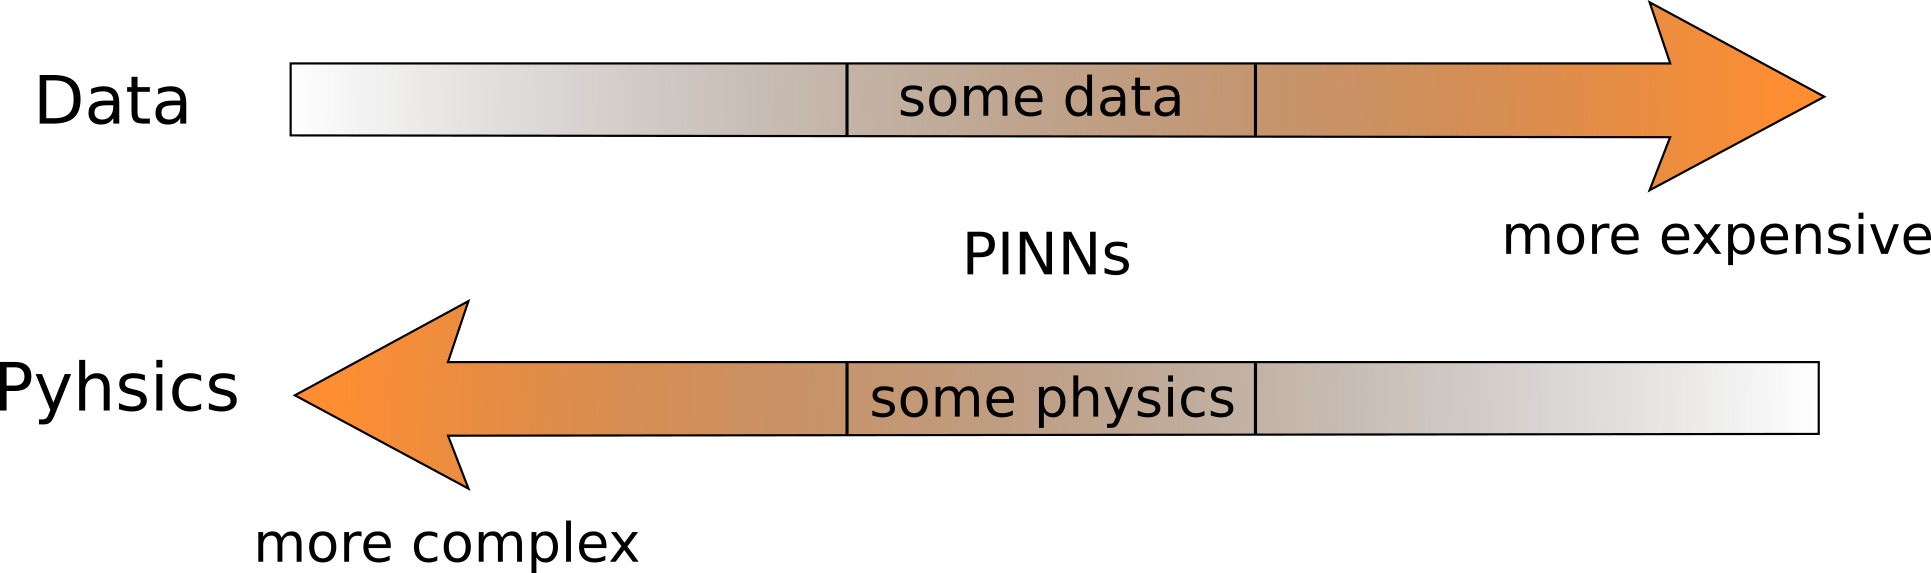
\includegraphics[scale=0.55]{data_physics.png}  
    \caption{Trade-off between data and physics}
    \label{fig:data_physics}
\end{figure}

 % Introduction
    \chapter{Physics-Informed Neural Networks (PINNs)}
\section{Overview}
\label{sec:pinns_overview}

Physics-informed neural networks can be considered as an alternative approach to conventional partial
differential equation (PDE) solvers. 
The general idea is to solve problems by minimizing the loss function constructed from PDEs where data
is limited. Compared to conventional solvers, PINNs

\begin{itemize}
    \item are mesh-free.
    \item can efficiently handle unstructured or irregular domains \cite{lu2021physics}.
    \item can be applied to solve also \textit{inverse} problems.
\end{itemize}

%-------------------------------------------------------------------------------------------------------------------
\section{Formulation of a PINN}
\label{sec:pinns_formulation}

\noindent Consider a partial differential equation as 

\begin{equation}
    \label{eq:governing}
    \frac{\partial u}{\partial t}+\mathcal{N}[u ; \lambda]=0, x \in \Omega, t \in [0,\mathcal{T}]
\end{equation}

\noindent where $u(t,x)$ is the latent solution with time $t \in [0,\mathcal{T}]$ and a spatial variable
$x \in \Omega$, $\mathcal{N}[u;\lambda]$ is the nonlinear differential operator
with the coefficient $\lambda$, and $\Omega$ is a subset of $\mathbb{R}^{D}$.

The conventional methods to solve Eq. \ref{eq:governing} are either analytical or numerical. The analytical solutions are 
not always feasible and numerical methods are expensive. The PINNs approach can be considered more feasible than analytical
methods and less expensive than numerical methods. 
The physics-informed neural network estimates the solution $u(t,x)$ and the physics-enhanced part evaluates
the given partial differential equation using the estimated solution. As shown in Fig. \ref{fig:pinn_arch}, the physics-informed
neural network predicts the solution $u(x,t)$ by using fully connected layers with nonlinear activation functions,
denoted as $\sigma$. The physics-enhanced part evaluates the chosen PDE, denoted as $f(x)$, using the higher derivatives
of the solution $u(x,t)$, denoted here $d_{x}, d_{xx}$ and $d_{t}$, with respect to space ($x$) and time ($t$), and the identity 
matrix of $u$. Since the solution is known on the boundaries and the approximated solution must fulfill the governing PDE, the loss
can be computed using a cost function, i.e. mean squared error. If the solution is not converged, the weights of the neural network
are updated using back-propagation to estimate the new solution, until the given convergence limit is reached. 


\begin{figure}[thbp]
    \centering
    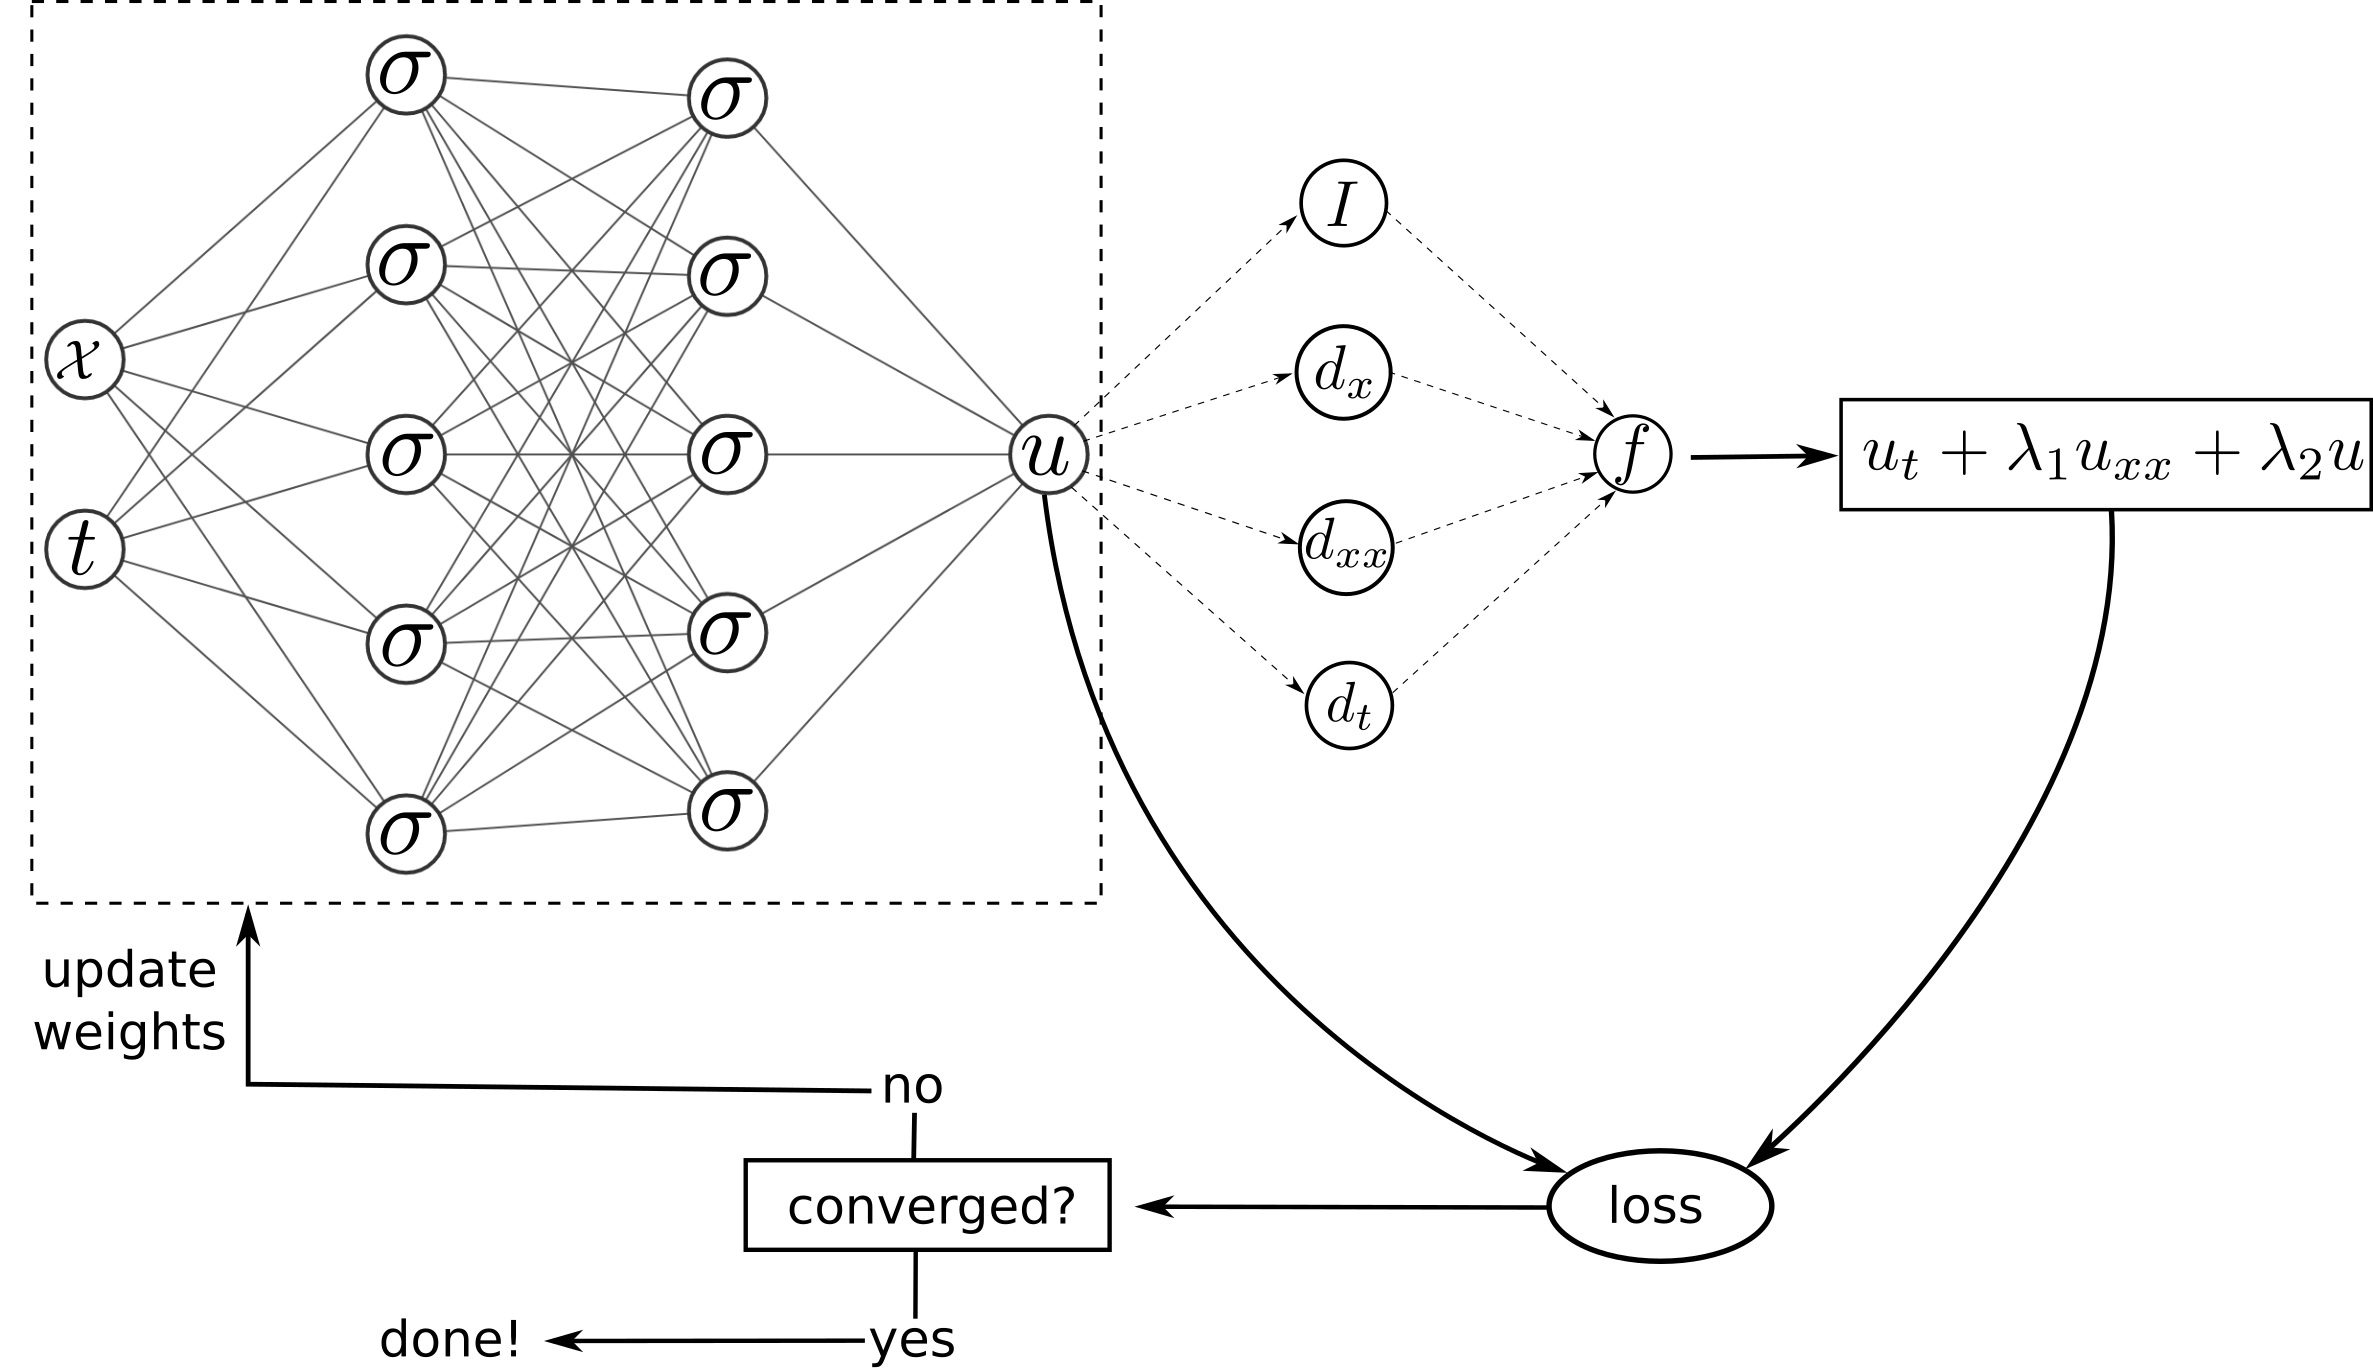
\includegraphics[scale=0.59]{pinn.png}  
    \caption{The visionary representation of physics-informed neural network for an arbitrary space-time dependent partial
    differential equation. }
    \label{fig:pinn_arch}
\end{figure}

Compared to classical neural networks, the loss function of a PINN has three terms:

\begin{equation}
    \label{eq:total_loss_compact}
    L = E_{u} +  E_{0} + E_{f}
\end{equation}

\noindent The first term, denoted as $E_{u}$, calculates the error for the approximated solution on the known
boundaries. In the case of a one dimensional non-linear heat equation subjected to the following 
homogenous Neumann boundary condition

\begin{equation}
    \label{eq:neumann}
    \frac{\partial u(x=1, t)}{\partial x}=h,
\end{equation}

\noindent the Dirichlet boundary condition

\begin{equation}
    \label{eq:dirichlet}
     u(x=0,t)=g,
\end{equation}

\noindent $E_{u}$ term is calculated as

\begin{equation}
    \label{eq:total_loss}
    E_{u} = E_{Neumann} + E_{Dirichlet},
\end{equation}

\noindent where

\begin{equation}
    \label{eq:Neumann_pinn}   
    E_{\text {Neumann}}=\frac{1}{N_{b}} \sum_{i=1}^{N_{b}}\left(\frac{\partial}{\partial x} u_{P}\left(x_{b}^{i}, t_{b}^{i} \right)-h\right)^{2}
\end{equation}

\noindent  enforces the homogenous Neumann boundary condition (refer to \ref{eq:neumann}) by penalizing the error between
the derivative of the predicted solution, denoted as $\frac{\partial}{\partial x} u_{P}\left(x_{b}^{i}, t_{b}^{i}\right)$, 
and the given Neumann
boundary condition $h$ at $N_{b}$ random
points $\left\{x_{b}^{i}, t_{b}\right\}_{i=1}^{N_{b}}$ on the boundary $x_{b} = 1$.

\noindent The term, $E_{Dirichlet}$ of the Eq. \ref{eq:total_loss}

\begin{equation}
    \label{eq:Dirichlet_pinn}      
    E_{\text {Dirichlet}}=\frac{1}{N_{b}} \sum_{i=1}^{N_{b}}\left(u_{P}\left(x_{b}^{i}, t_{b}^{i} \right)-g\right)^{2}
\end{equation}

\noindent enforces the Dirichlet boundary condition according Eq. \ref{eq:dirichlet}  by penalizing the error 
between approximated solution $u_{P}(x_{b}^{i}, t_{b}^{i})$ and prescribed Dirichlet boundary condition $g$ 
at $N_{b}$ random points $\left\{x_{b}^{i}, t_{b} \right\}_{i=1}^{N_{b}}$ on the boundary $x_{b} = 0$. 

\vspace{4mm}

\noindent The initial condition loss, $E_{0}$ of the Eq. \ref{eq:total_loss_compact}

\begin{equation}
    \label{eq:Initial_pinn}  
    E_{0}=\frac{1}{N_{0}} \sum_{i=1}^{N_{0}}\left(u_{P}\left(x_{0}^{i}, 0 \right)-u_{0}^{i}\right)^{2},
\end{equation}

\noindent with the following initial condition
\begin{equation}
    \label{eq:initial}
    u(x, t=0)=u_{0},
\end{equation}

\noindent enforces the initial conditions at $N_{0}$ random points 
$\left\{x_{0}^{i}, t_{b} \right\}_{i=1}^{N_{0}}$ at initial time $t_{b}=0$

\vspace{4mm}

The loss functions $E_{u}$ and $E_{0}$ contain only the loss on the known boundaries and
on the known initial conditions, respectively.

On the other hand, the final term of the Eq. \ref{eq:total_loss_compact}

\begin{equation}
    \label{eq:res_loss}   
    E_{\text {f}}=\frac{1}{N_{f}} \sum_{i=1}^{N_{f}}\left(\frac{\partial}{\partial t} u_{P}\left(x_{f}^{i}, t_{b}^{i} \right)-\mathcal{N}[u_{P}(x_{b}^{i}, t_{b}^{i})]\right)^{2}
\end{equation}

\noindent imposes the given partial differential equation at every random collocation point inside the domain by penalizing the estimated 
left-hand side and the known right-hand side of the governing equation. Since PINNs are mesh-free, the distribution of 
collocation points can be uniform or random.

After calculation of the loss terms, weights of the architecture is updated using back-propagation with the help of a optimization function,
i.e. stochastic gradient descent, Adam etc. 

\section{General remarks regarding PINNs}
\begin{itemize}
    \item A PINN is mesh-free so it can handle unstructured or irregular domains.
    \item PINNs can be deployed on both forward and inverse problems. In forward problems, they can find the hidden solution
    $u(x,t)$ 
    where the coefficients $\lambda$ are known (Eq. \ref{eq:governing}) or discover
    the parameters $\lambda$ using the provided solution, which are known as inverse problems. This approach
    is called also as data-driven identification.
    \item Depending on the type of the governing equation, they can be used on a wide variety of problems ranging from biological
    systems (reconstruction clinical magnetic resonance imaging (MRI) data) to the governing equations of continuum mechanics.
    \item Since the governing equations of the problem are involved in the learning process, PINNs can learn even data is limited.
    \item The derivatives of the network prediction $u_{P}$ with respect to space ($x$) and time ($t$) can be easily and
    efficiently computed by the automatic differentiation capabilities implemented in many deep learning tool kits, i.e. Tensorflow 
    \cite{abadi2016tensorflow} and 
    Pytorch \cite{NEURIPS20199015}.
    
\end{itemize}


















 
    \chapter{The Euler-Bernoulli Beam Theory with Governing Equations}
\label{sec:second}

A beam is a structural element having one dimension that is much larger than the other two and capable 
of resisting the loads applied laterally to the beam axis. Since the further investigations are pursued
for the Euler-Bernoulli beam theory, known as thin beam theory, the main assumptions and the governing 
equations of the Euler-Bernoulli are given in more detail.

\section{Assumptions of the Euler-Bernoulli Beams}

The main hypothesis of the Euler-Bernoulli beam theory is that plane cross-sections which are orthogonal 
to the beam axis (neutral axis) stay still plane and orthogonal to the beam axis after deformation. 
The overall assumptions of the Euler beam theory: %\ref{fig:euler_theory}

\begin{itemize}
    \item Plane cross-sections remain plane and perpendicular to the neutral axis of the beam after deformation.
    \item The deformations are small, so the equilibrium is computed on the reference configuration (Small deformation theory).
    \item Behavior of the beam is linear elastic and isotropic.
    \item Shear strains are neglected.
\end{itemize}


\begin{figure}[!ht]
    \centering
    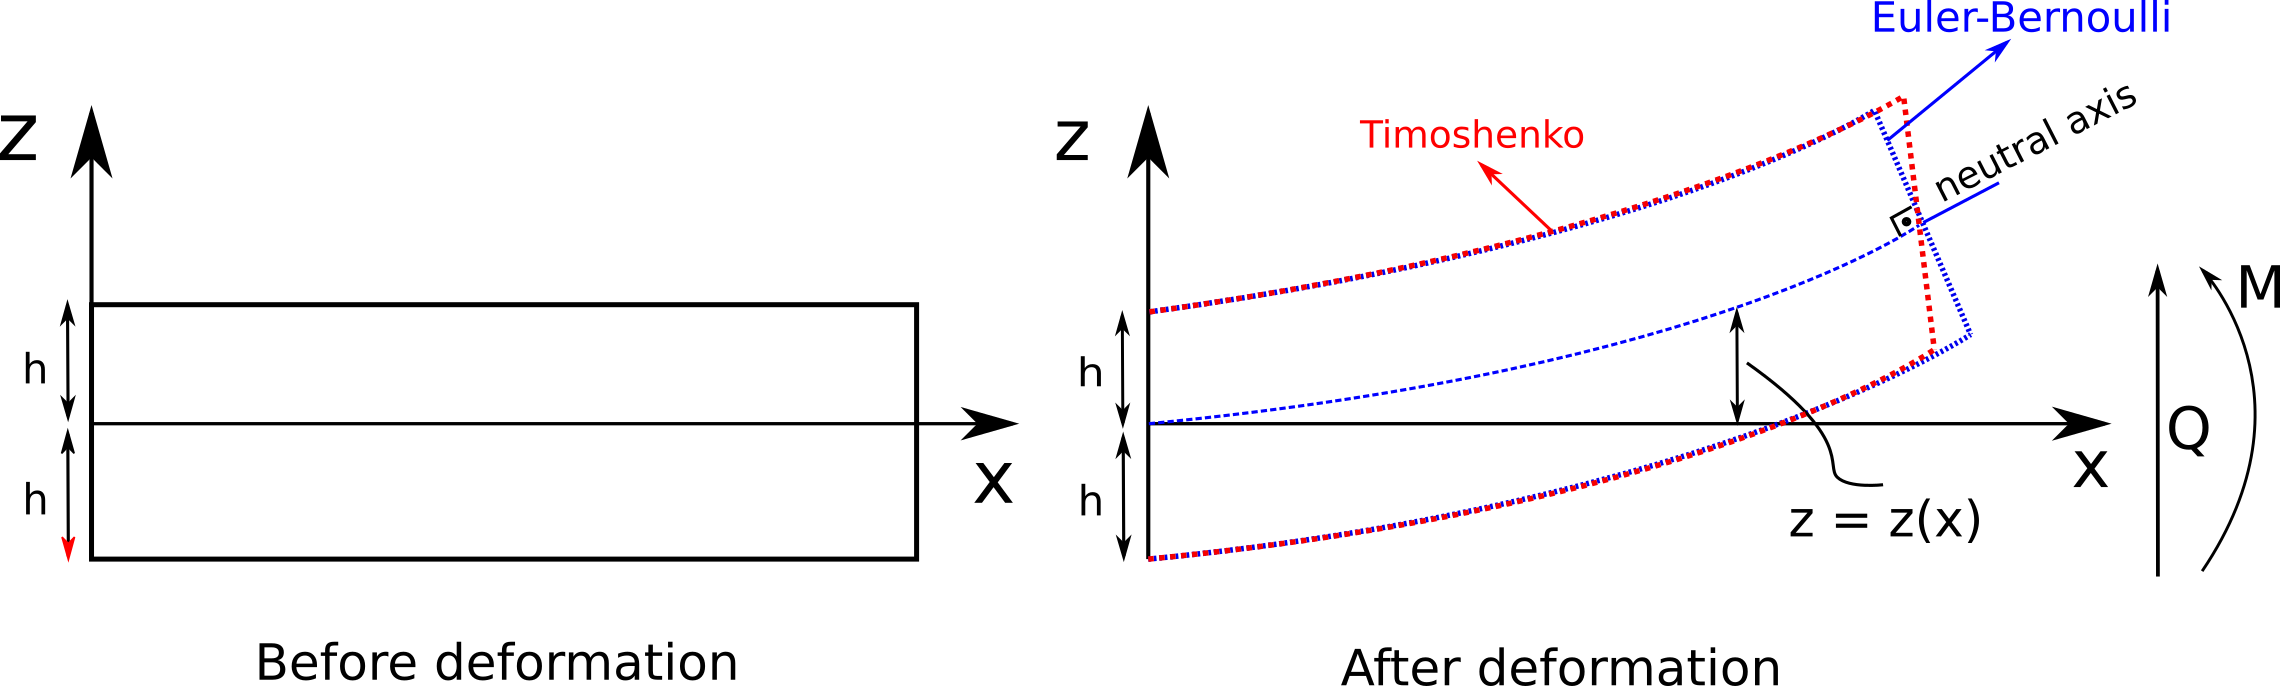
\includegraphics[scale=0.5]{beam_theory.png}  
    \caption{The Euler-Bernoulli and Timoshenko beam deflections}
    \label{fig:euler_theory}
\end{figure}

As depicted in Fig. \ref{fig:euler_theory}, the plane cross-sections stay plane and perpendicular to the 
beam axis in the Euler-Bernoulli beam. In the Timoshenko beam, plane cross-sections still remain plane but
are no longer perpendicular to the beam axis. The difference between normal to the beam axis and plane
cross-section is known as shear deformation. Here, shear strains will be ignored so the beam Formulation
is considered under the Euler-Bernoulli beam theory, which is known also as thin beam theory.

\section{Governing Equations}

\subsection{Time-dependent beam equation}

Consider the governing equation of an Euler-Bernoulli beam under 
the space-time dependent distributed load as (Fig. \ref{fig:beam_arbitrary})

\begin{equation}
    \label{eq:pde_time}
    \rho A \frac{\partial^{2} w(x,t)}{\partial t^{2}} + \frac{\partial^{2}}{\partial x^{2}}\left(E I \frac{\partial^{2} w(x,t)}{\partial x^{2}}\right) + q(x, t) = 0, x \in \Omega, t \in [0,T]
\end{equation}


\noindent where $w(x,t)$ is the unknown solution, $\Omega$ is a subset of $\mathbb{R}^{D}$,
$E$ is the uniform elastic modulus of the material, 
$I$ is the moment of the inertia of the cross-section of the beam, $\rho$
is the material density, $A$ is the cross-sectional area, and $q(x,t)$ is distributed space-time varying load. 
Eq. \ref{eq:pde_time} is known as also 
\textit{Euler-Langrange} equation \cite{wang2007vibration} used mainly in vibration problems. The first term
describes the dissipated kinetic energy where $\rho A$ is area density or the mass per unit length, 
and the second term characterizes the potential energy due to internal forces. 

\vspace{3mm}

\noindent The concentrated load $q$ can be considered as a special case of the distributed load as follows:

\begin{equation}
    \label{eq:load_time}
    q(x,t) = P(t)\delta\left(x-x_{0}\right)
\end{equation}

\noindent where $\delta$ is the \textit{Dirac} delta function, and $P(t)$ is the time-dependent load applied
at position $x_{0}$.



\begin{figure}[!ht]
    \centering
    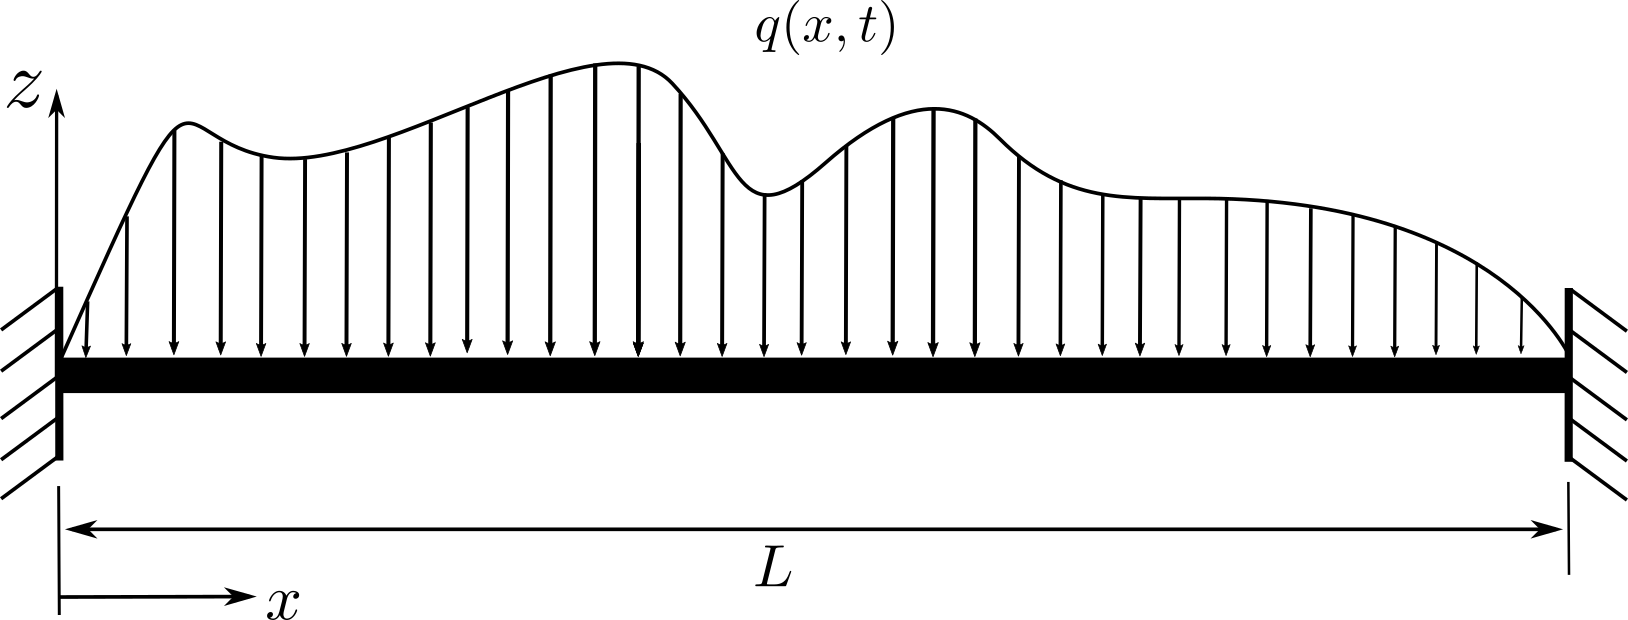
\includegraphics[scale=0.7]{beam_arbitrary.png}  
    \caption{A fixed-fixed supported beam under a space-time dependent distributed load.}
    \label{fig:beam_arbitrary}
\end{figure}

\subsection{Static beam equation}

Eliminating time terms in Eqs. \ref{eq:pde_time} and \ref{eq:load_time}, the governing ordinary differential equation
is obtained for a static model

\begin{equation}
    \label{eq:ode_space}
    \frac{\partial^{2}}{\partial x^{2}}\left(E I \frac{\partial^{2} w(x)}{\partial x^{2}}\right) + q(x) = 0, x \in \Omega,
\end{equation}

\noindent and, similarly if $q(x)$ is a concentrated load

\begin{equation}
    q(x) = P \delta\left(x-x_{0}\right).
\end{equation}


\section{Boundary Conditions and Beam Supports}

To estimate the unknown solution $w(x,t)$, 
the governing equation of the Euler-Bernoulli beam 
must be solved using the initial and boundary conditions. Since the governing equation is of the $4th$ order in space (Eq. \ref{eq:pde_time}), 
four different boundary conditions are introduced:
\begin{itemize}
    \item $w(x,t) \rightarrow$ represents the displacement in the z direction,
    \item $w_{x}(x,t) \rightarrow$ indicates the slope of the beam,
    \item $w_{xx}(x,t) \rightarrow$ measures the bending moment,
    \item $w_{xxx}(x,t) \rightarrow$ measures the shear force, 
\end{itemize}

\noindent at location $x \in \Omega$ and time $t \in [0,T]$. 

Similary, and two initial conditions are needed as Eq. \ref{eq:pde_time} is of the $2^{th}$ order in time
\begin{itemize}
    \item $w(x,0) \rightarrow$ represents the displacement in the z direction,
    \item $w_{t}(x,0) \rightarrow$  indicates the time derivative of the displacement,
\end{itemize}

\noindent at location $x \in \Omega$ and at time $t=0$. Initial conditions are not taken 
into account in the static beam equation since the time-dependent derivative term vanishes. 

\vspace{5mm}
\noindent Two main supports will be further investigated:
\begin{itemize}
    \item fixed supported beams
    \item simply supported beams
\end{itemize}

\subsection{Cantilever beam}

A cantilever beam is fixed supported at one end and free at the other as depicted in Fig. \ref{fig:beam_cantilever}. 
No displacement and rotation are allowed at the fixed edge. No bending moment and no shear force at the free edge
are generated. 

\begin{figure}[!ht]
    \centering
    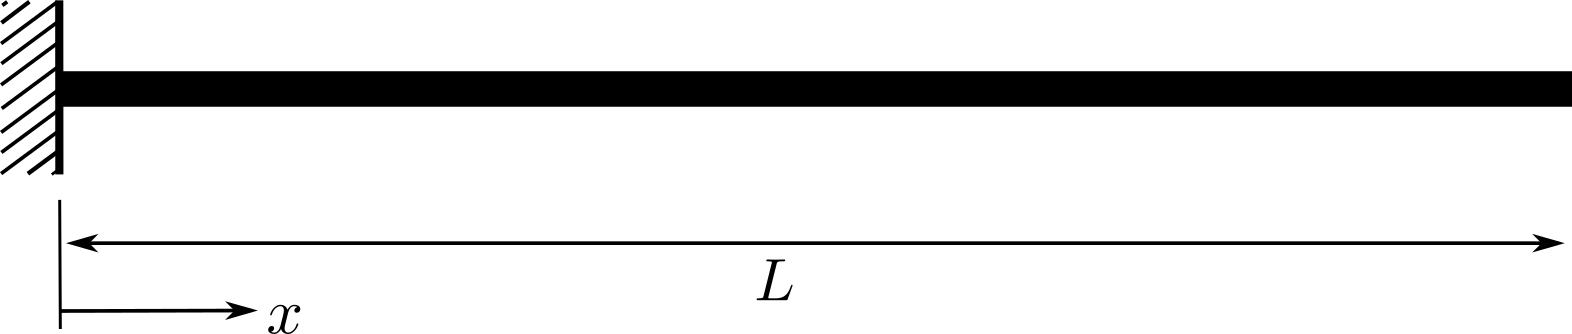
\includegraphics[scale=0.6]{beam_cantilever.png}  
    \caption{An illustration of a fixed supported beam}
    \label{fig:beam_cantilever}
\end{figure}

Boundary conditions of a cantilever beam
\begin{equation}
    \begin{array}{l}
    w(x,t)=0 \quad and \quad w_{x}(x,t)=0, \quad at \; x=0, t=[0,T] \\
    w_{xx}(x,t)=0 \quad and \quad w_{xxx}(x,t)=0, \quad at \; x=L, t=[0,T]
    \end{array}
\end{equation}

\subsection{Simply supported beam}
Simply supported beam is pinned at the ends for two edges as shown in Fig. \ref{fig:beam_pinn}. At both pinned ends, 
no displacement but rotation 
is allowed which means that no bending moments are generated.

\vspace{5mm}

\begin{figure}[!ht]
    \centering
    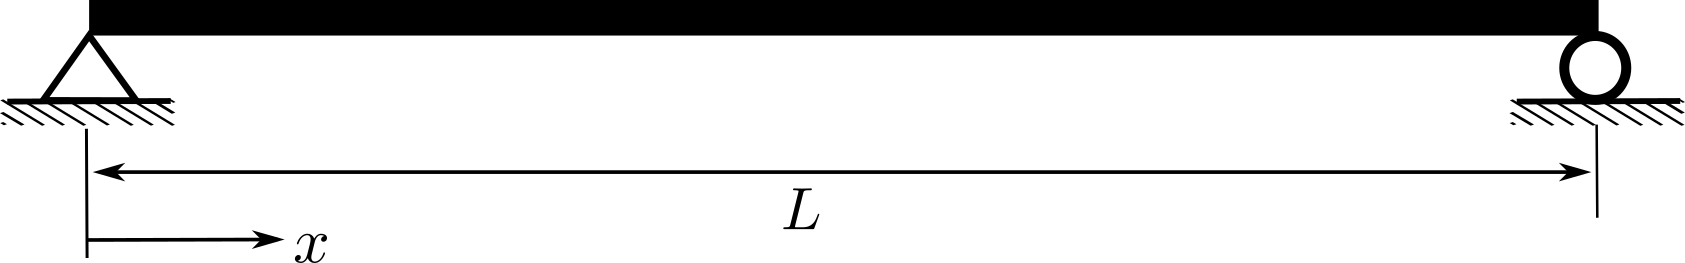
\includegraphics[scale=0.6]{beam_pinn.png}  
    \caption{An illustration of a simply supported beam.}
    \label{fig:beam_pinn}
\end{figure}

Boundary conditions of a simply supported beam
\begin{equation}
    \label{eq:simply_supported_bc}
    \begin{array}{l}
    w(x,t)=0 \quad and \quad w_{xx}(x,t)=0, \quad at \; x=0, t=[0,T] \\
    w(x,t)=0 \quad and \quad w_{xx}(x,t)=0, \quad at \; x=L, t=[0,T]
    \end{array}
\end{equation}

\subsection{Clamped beam}
A clamped beam is fixed supported at both ends as depicted in Fig. \ref{fig:beam_clamped}. At both fixed ends,
no displacement and rotation is allowed. 

\begin{figure}[!ht]
    \centering
    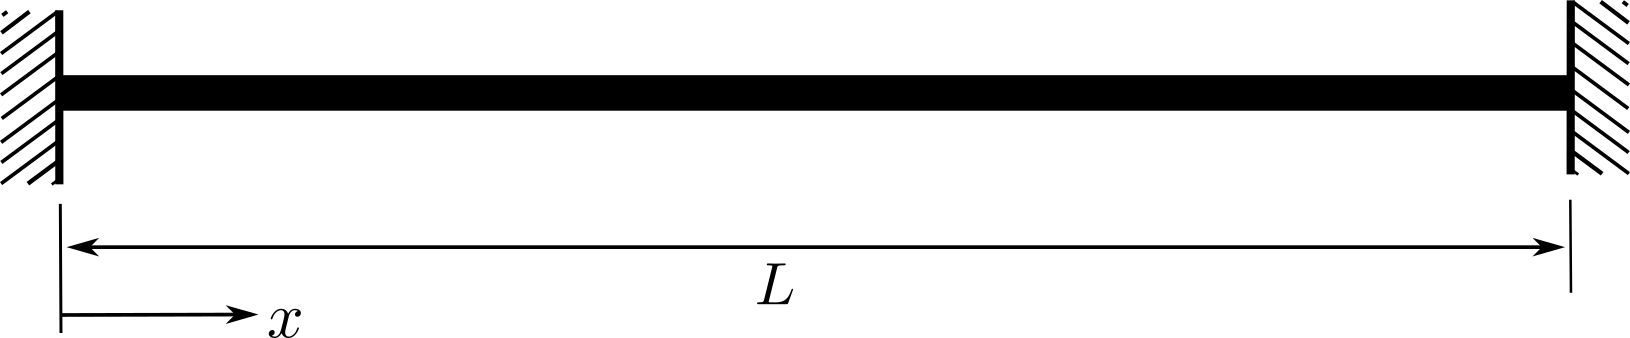
\includegraphics[scale=0.6]{beam_clamped.png}  
    \caption{An illustration of a clamped beam.}
    \label{fig:beam_clamped}
\end{figure}

Boundary conditions of a clamped beam
\begin{equation}
    \begin{array}{l}
    w(x,t)=0 \quad and \quad w_{x}(x,t)=0, \quad at \; x=0, t=[0,T] \\
    w(x,t)=0 \quad and \quad w_{x}(x,t)=0, \quad at \; x=L, t=[0,T]
    \end{array}
\end{equation}
 % The beam theory with governing equations
    \chapter{Application of PINNs on 1D Beams}
In Sec. \ref{sec:pinns_formulation}, a general formulation for physics-informed neural networks is explained. 
Here, one-dimensional Euler-Bernoulli beams under the distributed load with uniform geomerical and material properties
are conducted, which are governed by an ordinary differential equation (Eq. \ref{eq:ode_space}) in static models and 
governed by a partial differential equation (Eq. \ref{eq:pde_time}) in continuous-time models.   
\label{sec:third}

\section{Static Models}
Consider the governing equations of one-dimesional linear elastic Euler-Bernoulli 
beam (Fig. \ref{fig:beam_clamped}) with the corresponding boundary conditions of clamped beam as

\begin{equation}
    \label{eq:static_beam_1}
    \frac{\partial^{2}}{\partial x^{2}}\left(E I \frac{\partial^{2} w(x)}{\partial x^{2}}\right)+q(x)=0 \quad \text { on }\Omega
\end{equation}

\begin{equation}
    \label{eq:static_beam_2}
    \frac{\partial w(x)}{\partial x} = h \quad \text { on } \Gamma_{N},
\end{equation}

\begin{equation}
    \label{eq:static_beam_3}
    w(x) = g \quad \text { on } \Gamma_{D}.
\end{equation} 

\noindent The Neumann and Dirichlet boundary conditions are denoted as $\Gamma_{N}$ and $\Gamma_{D}$. To give a better understanding, 
the spatial domain is defined $\Omega=[0,L]$, with $\Gamma_{D}= \{x | x = 0, x = L\}$ and $\Gamma_{N}= \{x | x = 0, x = L\}$. 
If the length of the beam is set to $L=1$, the following boundary conditions 
of a clamped support Euler-Bernoulli beam are obtained

\begin{equation}
    \begin{aligned}
    \label{eq:static_beam_4}
    w(x=0)=0 & \text { and } & w_{x}(x=0)=0, \\
    w(x=1)=0 & \text { and } & w_{x}(x=1)=0.
    \end{aligned}
\end{equation}

The physics-informed neural network approximates the unknown solution $w(x)$
through the hidden layers enhanced with non-linear activation functions $\sigma$ using the spatial domain $x$ as the input 
as depicted in Fig. \ref{fig:pinn_static_beam}.
Since only the solution on the boundaries are known, the predicted solution for every location inside the domain must fulfill
the Eq. \ref{eq:static_beam_1} such that 

\begin{equation}
    \label{eq:f_static}
    f:=\frac{\partial^{2}}{\partial x^{2}}\left(E I \frac{\partial^{2} w(x)}{\partial x^{2}}\right)+q(x).
\end{equation}

Here the $f$ term represents the residuum or physics-informed residual which has to be fulfilled at every point inside
the domain. The main purpose of PINNs is to minize the residuum enforcing the boundary conditions via the loss function.

Combining Eqs. \ref{eq:static_beam_4} and \ref{eq:f_static} with \ref{eq:Neumann_pinn}, 
\ref{eq:Dirichlet_pinn}, \ref{eq:res_loss}, \ref{eq:total_loss} and \ref{eq:total_loss_compact}, the loss function of 
static clamped Euler-Bernoulli beam is defined

\begin{equation}
    \label{eq:app_static_overall_loss}
    \begin{aligned}
        L & = E_{u} +  E_{f} \\ 
          & = E_{Neumann} + E_{Dirichlet} + E_{f} \\ 
          & = \frac{1}{N_{b}} \sum_{i=1}^{N_{b}}\left[\left(\frac{\partial}{\partial x} w_{P}\left(x_{b}^{i}\right)-h\right)^{2} +
          \left( w_{P}\left(x_{b}^{i}\right)-g\right)^{2} \right] + 
          \frac{1}{N_{f}} \sum_{i=1}^{N_{f}}\left(f_{P} (x_{f}^{i})\right)^{2} \\
          & = \frac{1}{N_{b}} \sum_{i=1}^{N_{b}}\left[\underbrace{\left(\frac{\partial}{\partial x} w_{P}\left(x_{b}^{i}\right)\right)^{2}}_{\text{Neumann term}} +
          \underbrace{ \vphantom{\left(\frac{\partial}{\partial x}\right)} \left( w_{P}\left(x_{b}^{i}\right)\right)^{2}}_{\text{Dirichlet term}} \right] + 
          \frac{1}{N_{f}} \sum_{i=1}^{N_{f}}\left(f_{P} (x_{f}^{i})\right)^{2}
    \end{aligned}
\end{equation}

\noindent The $h$ and $g$ terms
are the prescribed Neumann and Dirichlet boundary conditions at $N_{b}$ 
boundary points $\left\{x_{b}^{i}\right\}_{i=1}^{N_{b}} = \left\{0,1\right\}$. 
Since the beam is considered as a clamped beam, $h=0$ and $g=0$.  
The last term of Eq. \ref{eq:app_static_overall_loss} minizes the error at every point inside the spatial domain,
called as the collocation 
points $\left\{x_{f}^{i}\right\}_{i=1}^{N_{f}}$. The collocation points can be generated using random or uniform distributions.

\begin{figure}[!ht]
    \centering
    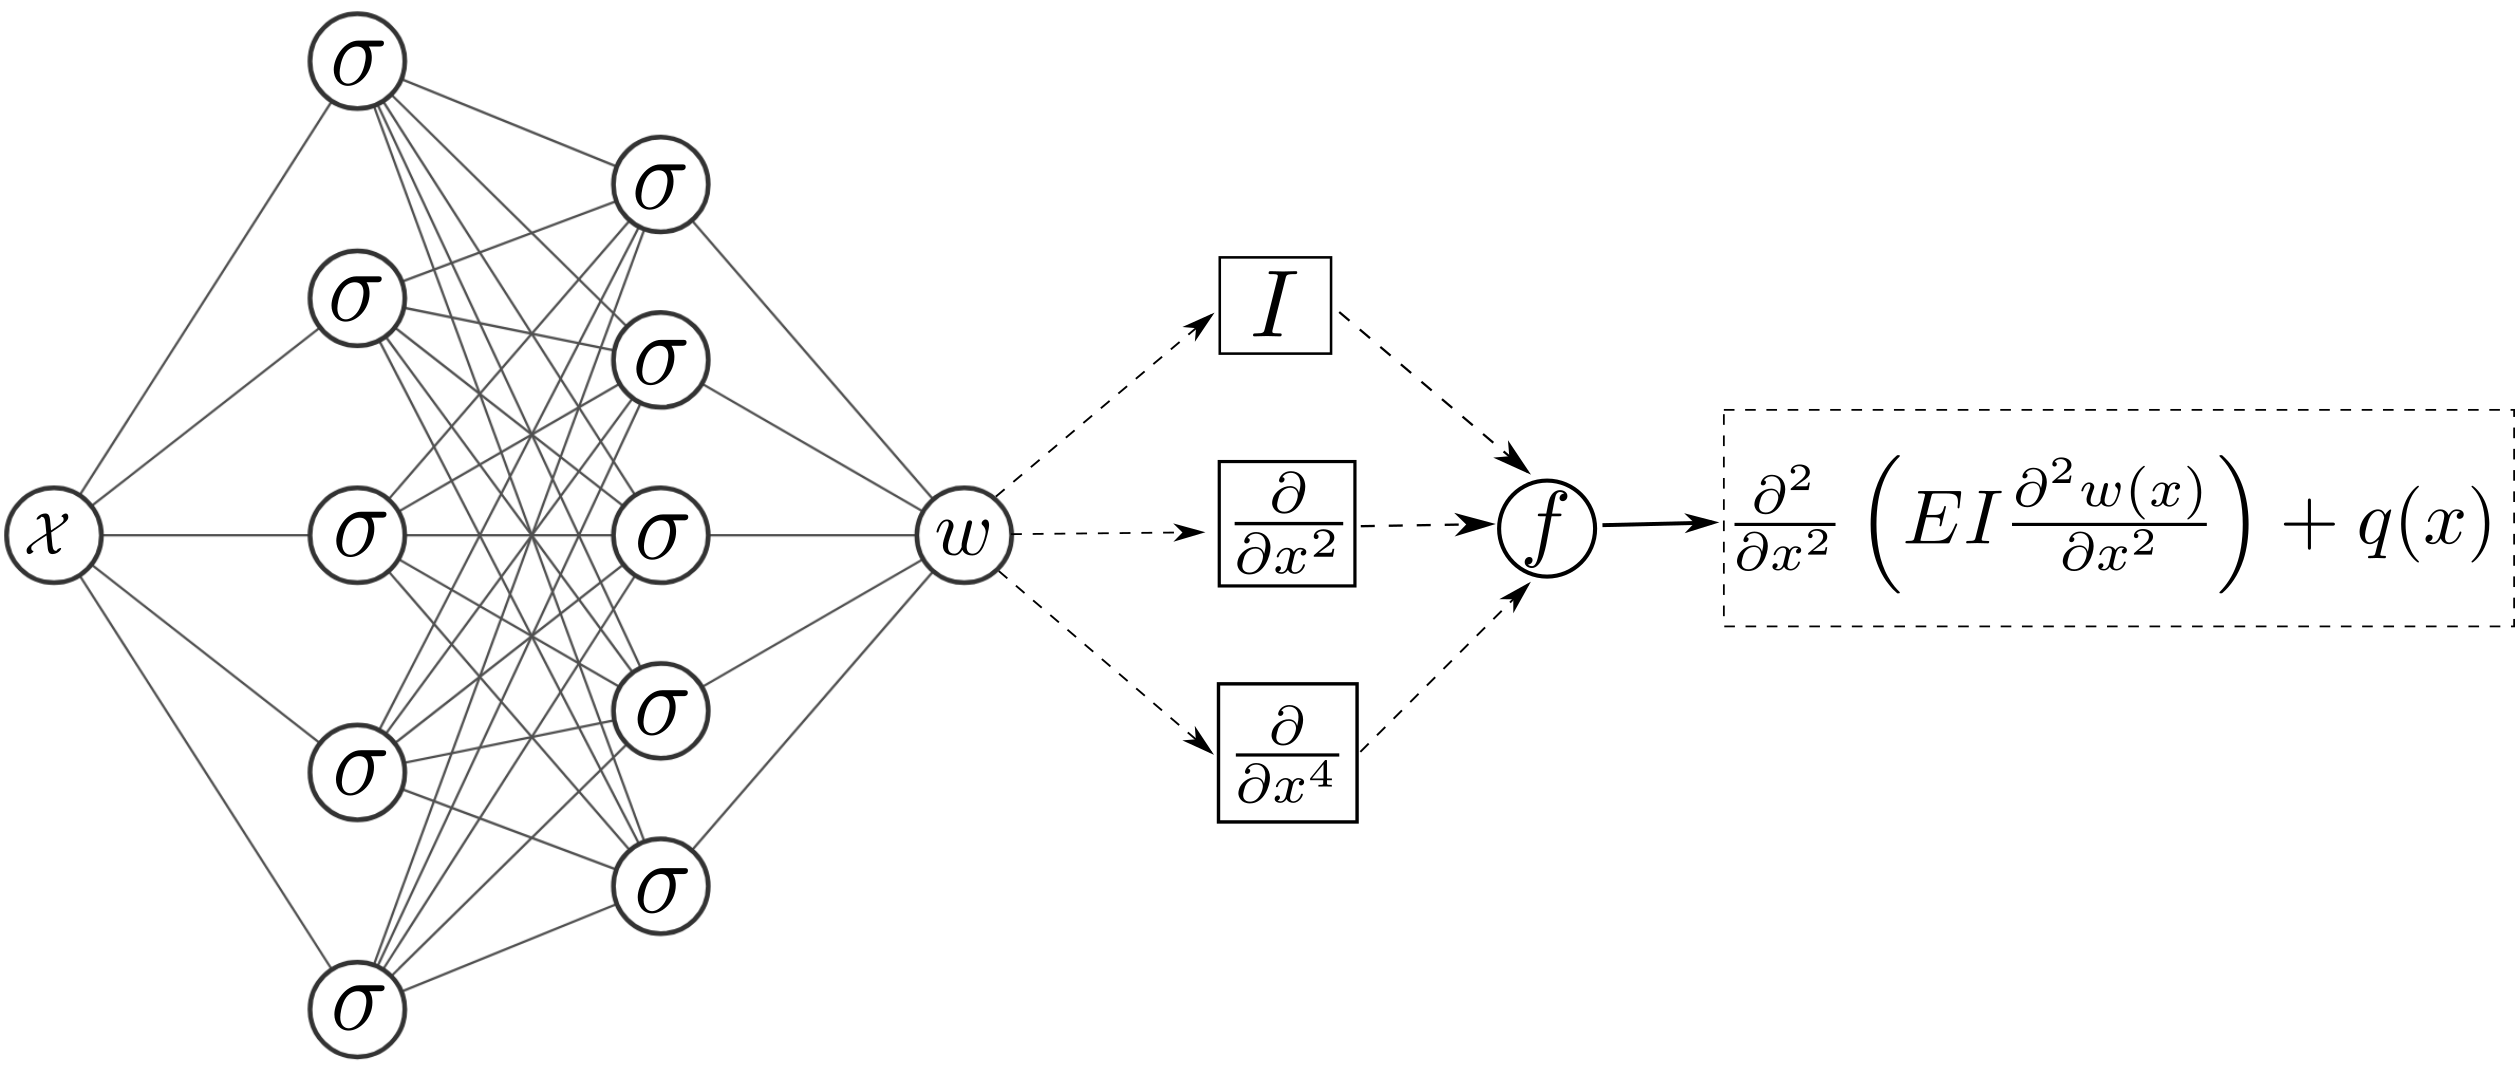
\includegraphics[scale=0.55]{pinn_static_beam.png}  
    \caption{An illustration of physics-informed neural network for the governing ordinary differential
    equation of the one-dimensional Euler-Bernoulli beam.}
    \label{fig:pinn_static_beam}
\end{figure}

For demonstrating the application of PINNs on the Euler-Bernoulli beams, three cases are further
investigated to involve the higher-order derivatives in the loss function as depicted 
in Fig. \ref{fig:beam_app_models}. For instance,
the clamped beam contains only the first order, while the cantilever beam contains the first, 
second and third-order derivatives (cf. \ref{fig:beam_cantilever}, \ref{fig:beam_pinn},
\ref{fig:beam_clamped}). For simplicity, Young's modulus and the moment of inertia terms are
set to $AE=1$, the beam length and the magnitude of the distributed loading are set to $L=1$ and $q=1$, relatively.

\vspace{5mm}
The following PINN architecture is used to compute the approximated solution:
\begin{itemize}
    \item Architecture contains 1 input layer, 1 output layer and 3 hidden layers
    containing 30 nodes.
    \item Hyperbolic tangent activation functions $tanh$ are used to non-linearize the outputs of the layers.
    \item The \textit{Glorot Uniform} initializer is applied to initialize the weights randomly to
    avoid dying out of the nodes.
    \item The \textit{Adam} optimizer with learning rate \textit{0.0005} is chosen as the optimization function.
    \item The number of collocation points is set $N_{f}=20$ and the Sobol sampling
    is performed to have a non-uniform distribution. 
\end{itemize}


\begin{figure}[!ht]
    \centering
    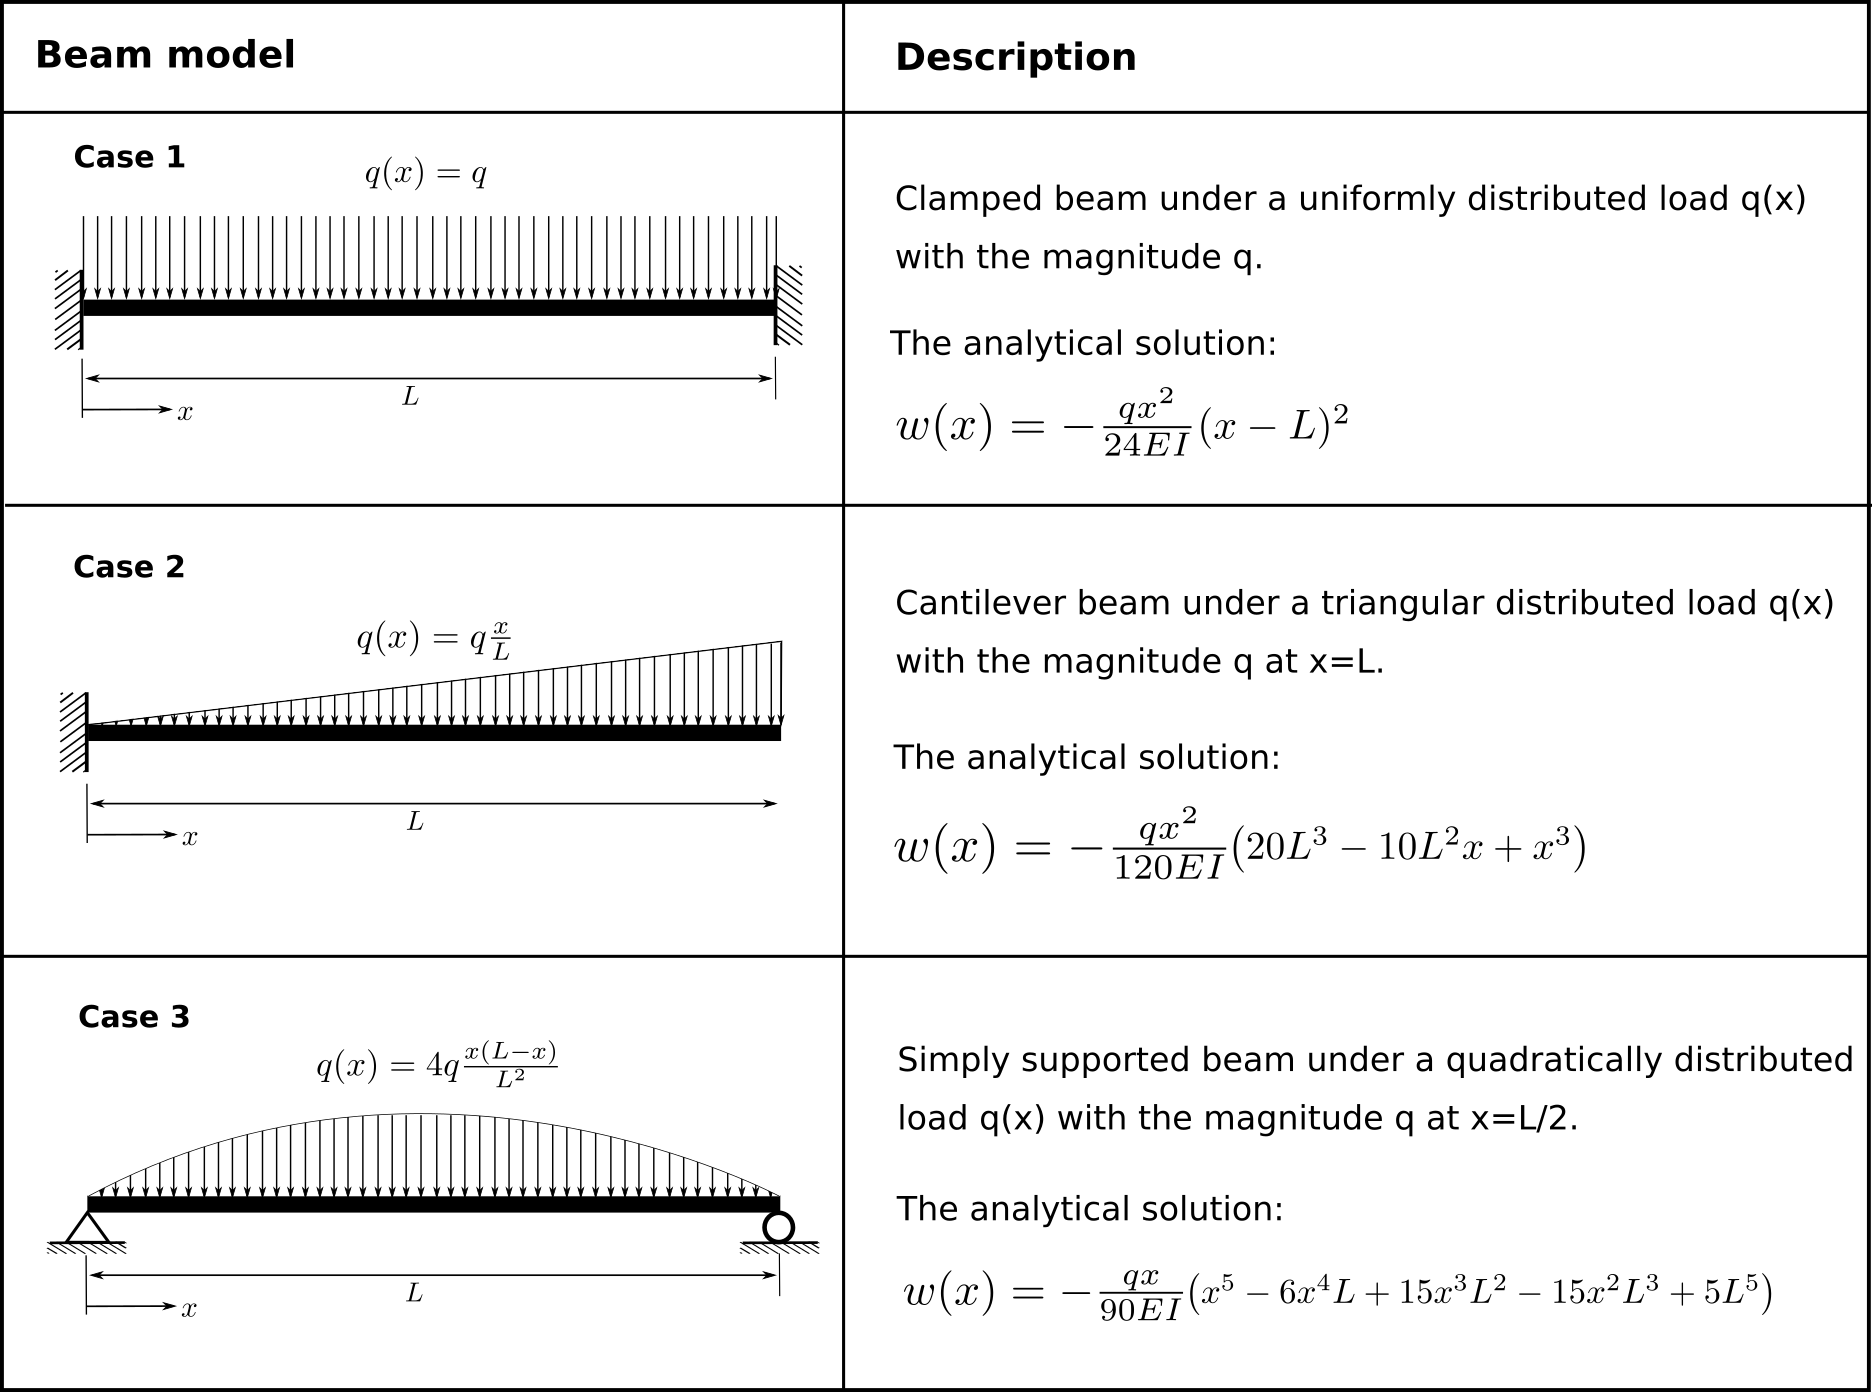
\includegraphics[scale=0.8]{beam_app_models.png}  
    \caption{Three investigated beam models with their descriptions and analytical solutions.}
    \label{fig:beam_app_models}
\end{figure}

The results of the investigated cases are given in Fig. \ref{fig:static_res}. Figures on the left show that the
predicted displacements are almost identical to the analytical solutions at each collocation point as can be seen
in the magnitude of the loss function. On the other hand, there is a difference in terms of the order of magnitudes
of the loss functions between the differential equation loss and the total boundary losses. 
The reason is that the boundary conditions are not explicitly enforced. In Eq. \ref{eq:app_static_overall_loss}, 
the boundary condition losses are added to overall lost and this overall loss is minimized. To enforce the boundary
conditions, the loss function can be reformulated to a soft constraint problem or penalty methods can be considered
\cite{lu2021physics}.     

\begin{figure}[t]
    \centering
    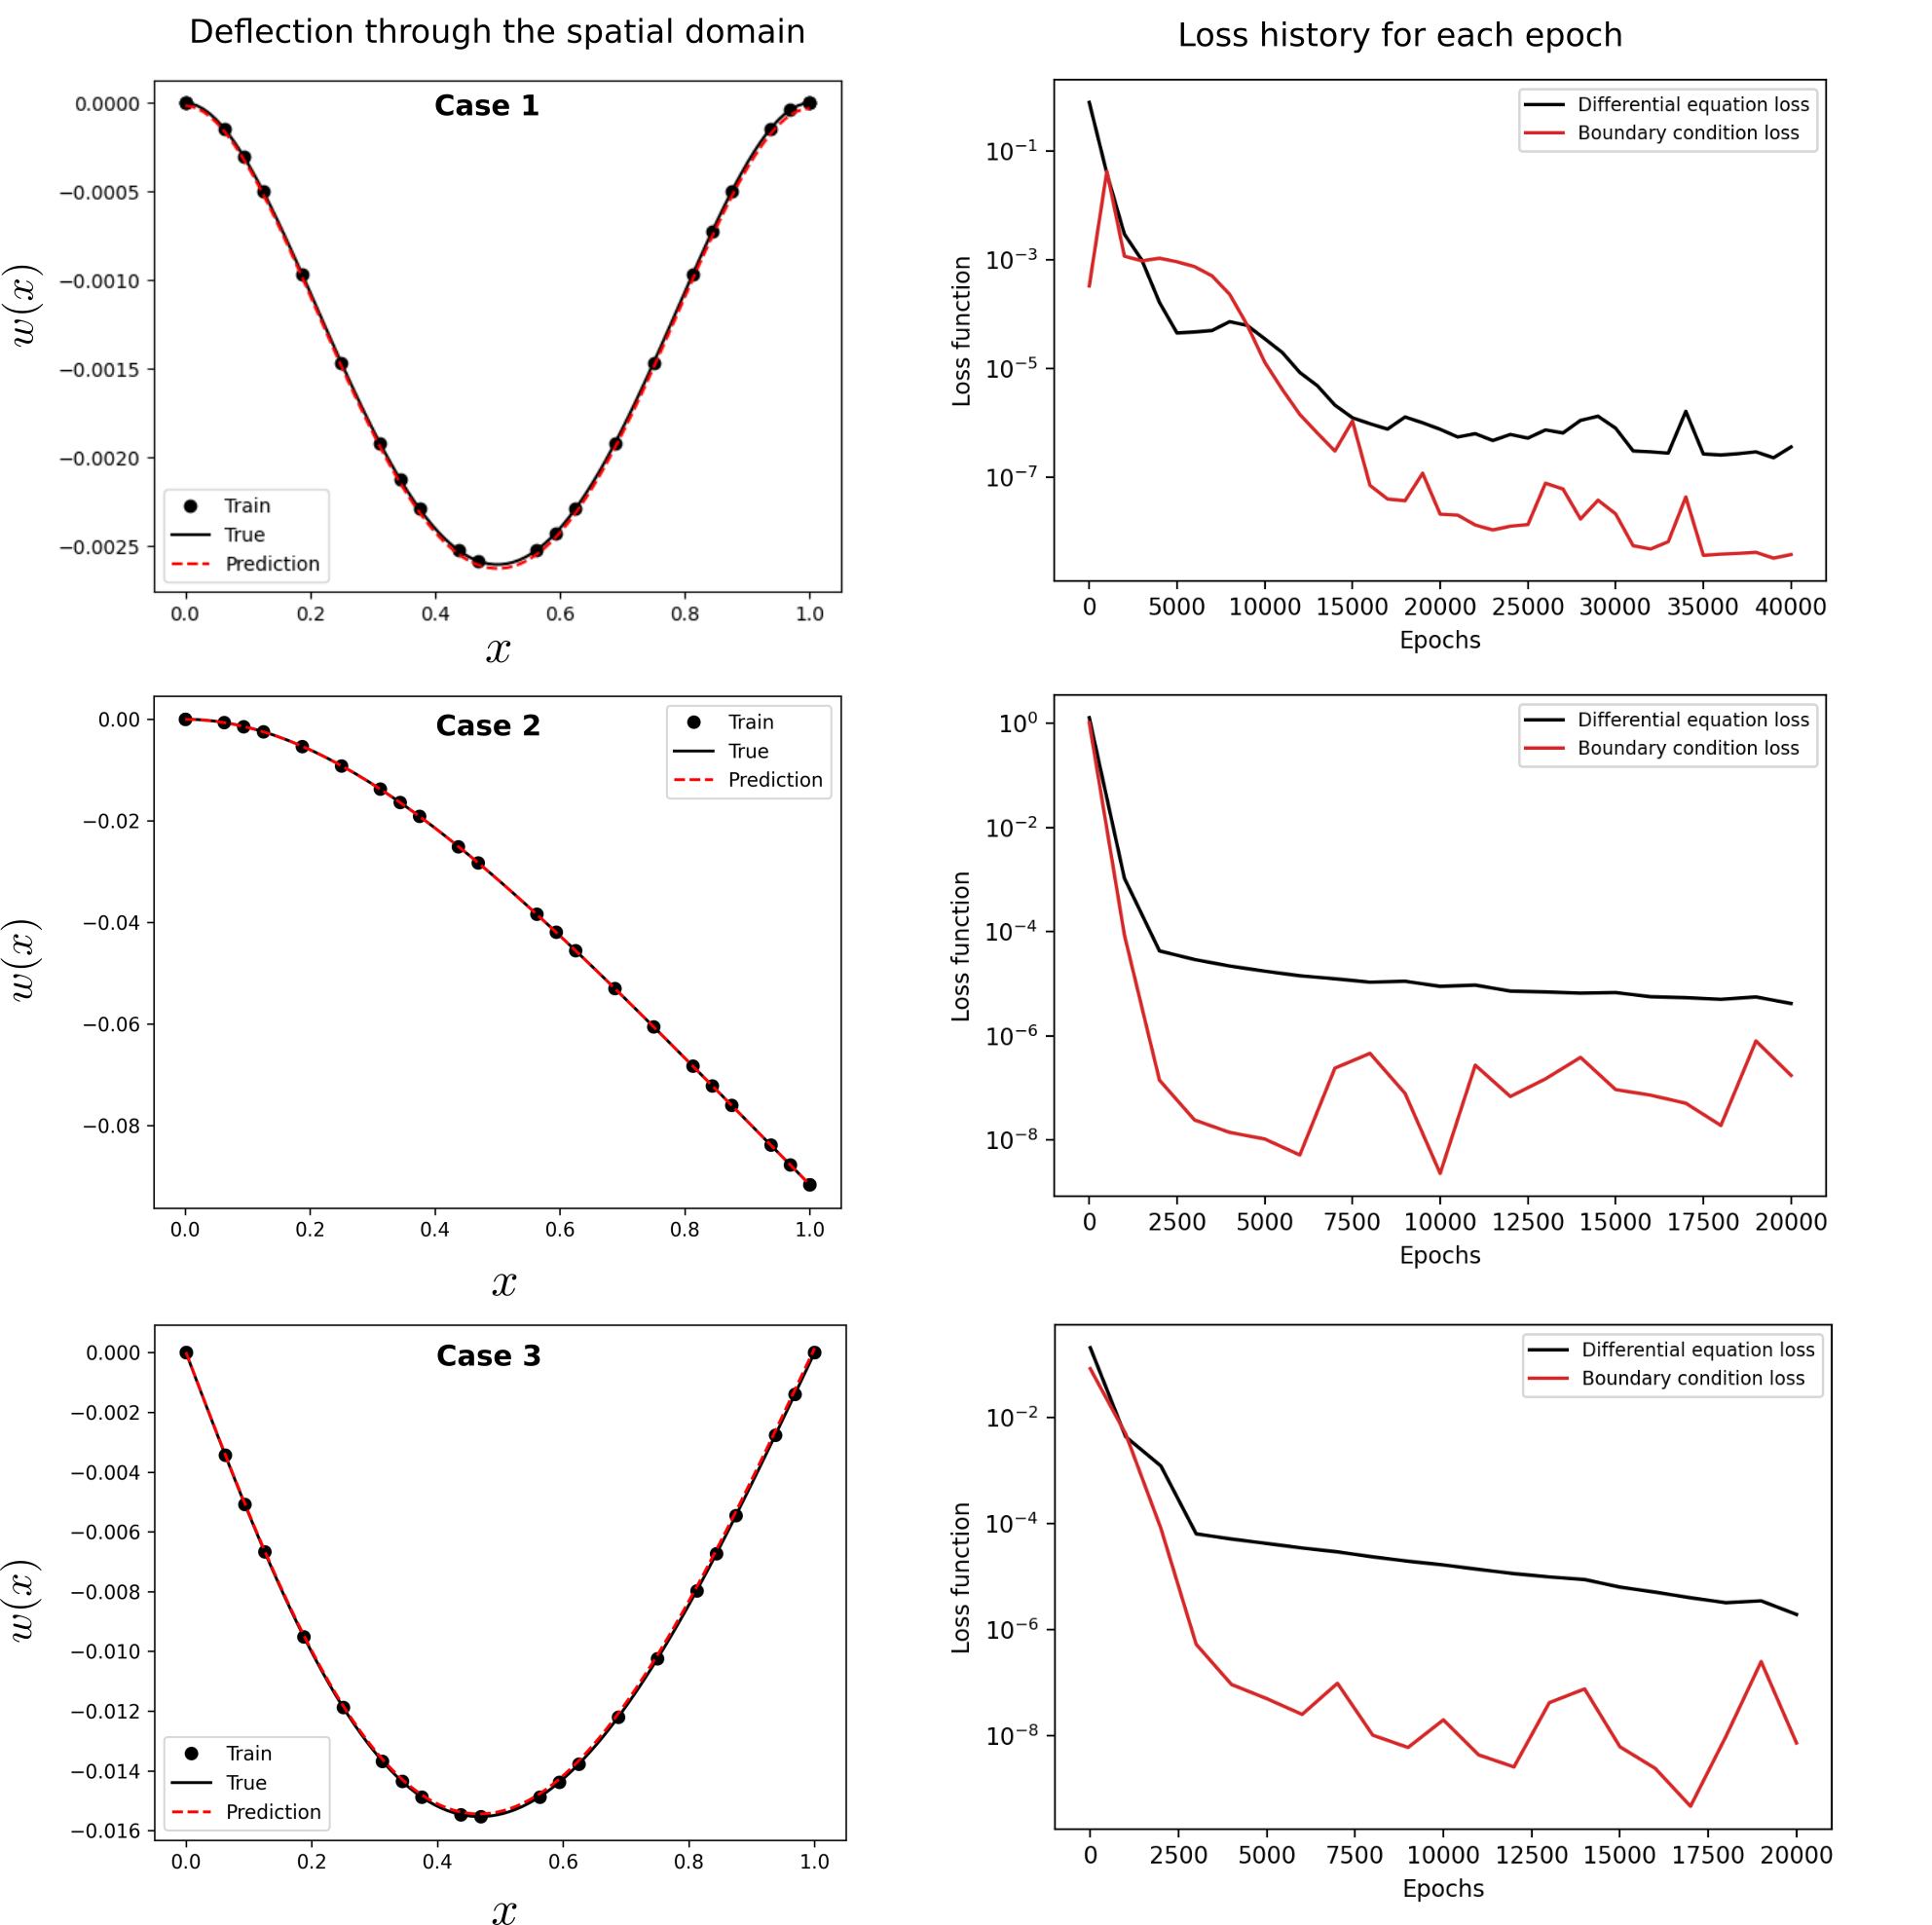
\includegraphics[scale=0.75]{static_res.png}  
    \caption{On the figures left, the predicted and true deflections through the spatial domain are compared for
    three different cases. On the figures right, the loss history containing the differential equation and
    boundary condition losses are given for each epoch.}
    \label{fig:static_res}
\end{figure}

\clearpage

\subsection{A complex consideration}

So far, simple beam structures with uniform material and geometrical properties under non-complex
loadings have been investigated. Consider a simply supported beam having the following non-uniform cross-section 

\begin{equation}
    I(x) = \left( \frac{x}{L} \right)^{2}
\end{equation}

under the following loading
\begin{equation}
    p(x)=\frac{8\pi^{2}\left(\left(2 \pi^{2} x^{2}-L^{2}\right) \sin (\frac{2 \pi x}{L})-4 \pi x \cos (\frac{2 \pi x}{L})\right)}{L^{4}},
\end{equation}


as depicted in Fig. \ref{fig:beam_complex}. Applying the boundary conditions (Eq. \ref{eq:simply_supported_bc})
and using the governing equation of the beam theory (\ref{eq:static_beam_1}), the analytical solution is obtained

\begin{equation}
    w(x) = \sin (\frac{2\pi x}{L}).
\end{equation}

For simplicity, Young's modulus is set to $E=1$ and the length of the beam is set to $L=1$. 

\begin{figure}[!hb]
    \centering
    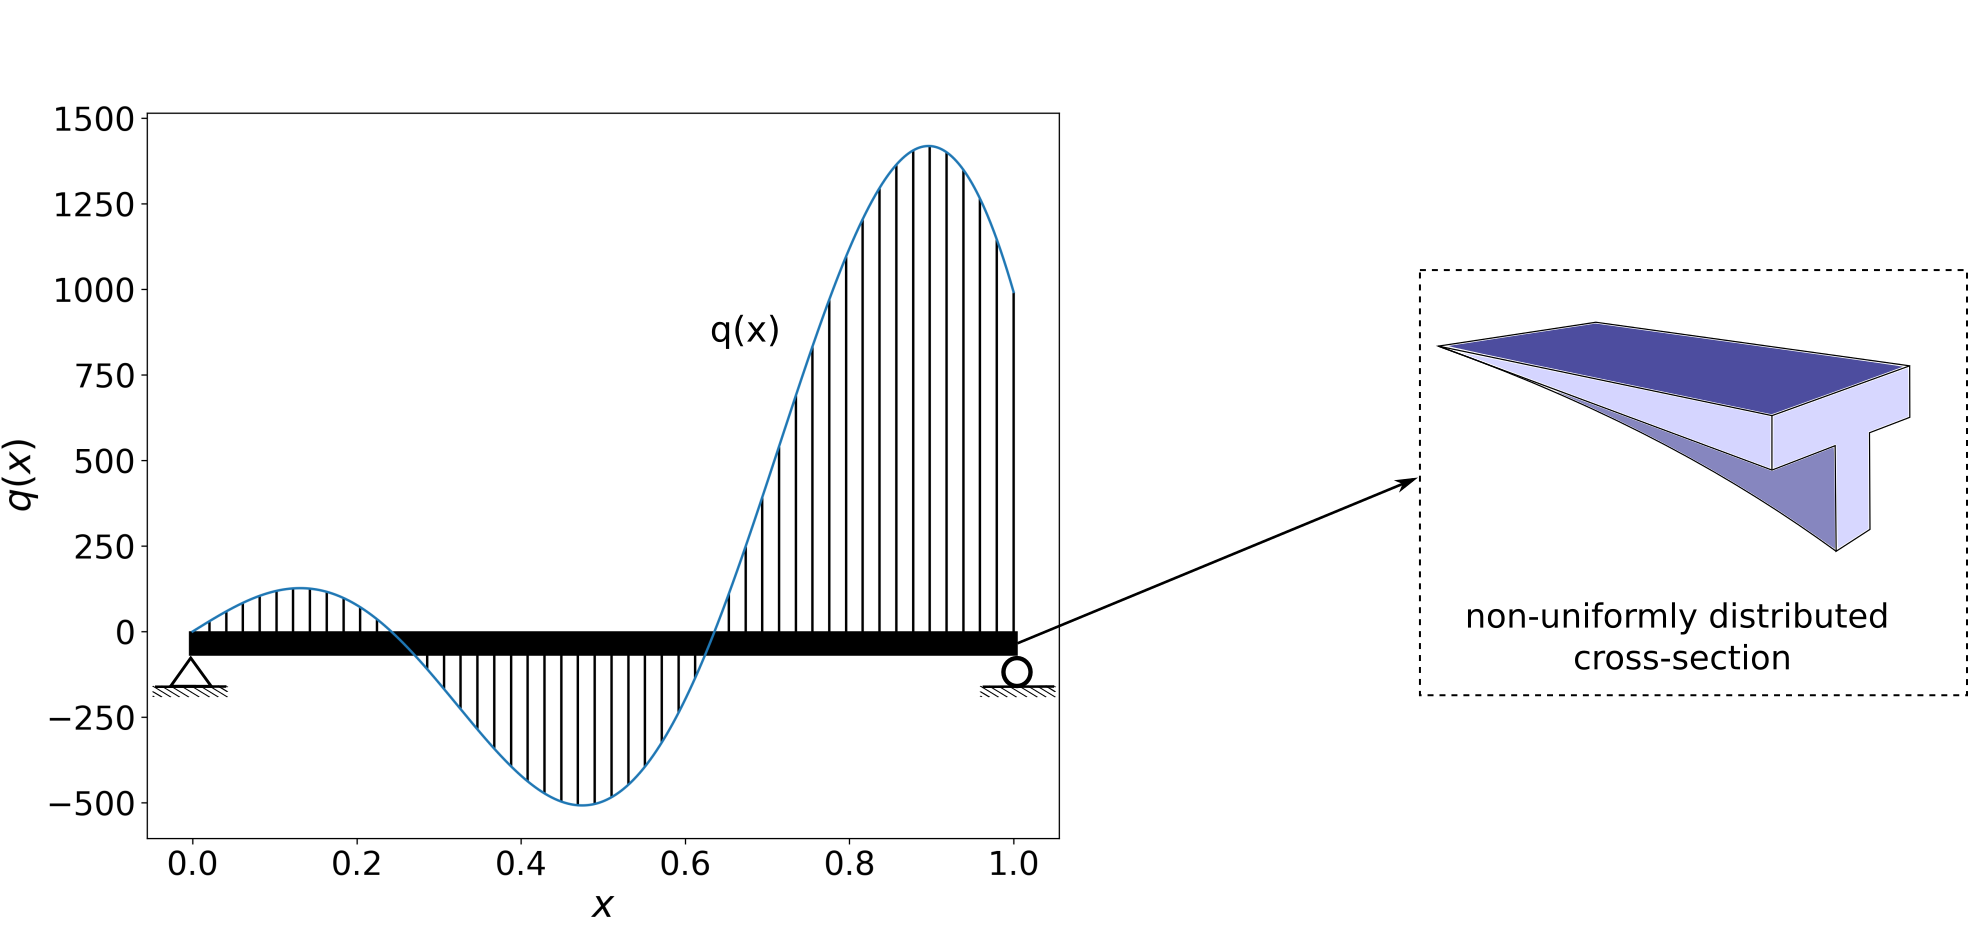
\includegraphics[scale=0.70]{beam_complex.png}  
    \caption{An illustration of a simple supported beam having non-uniformly distributed cross-section under an arbitrary load}
    \label{fig:beam_complex}
\end{figure}


The results of the investigated complex model is given Fig. \ref{fig:res_complex}. Similar to the previously 
conducted simpler models, 
figure on the left shows that the predicted displacements are almost identical to the true solution. 
On the contrary, the difference between differential equation loss and boundary equation loss is large compared
to the simple models (see \ref{fig:static_res}). The difference is due to the magnitude of the quantities. 
Since the applied load has a large magnitude compared to the predicted displacement, the initial differential loss
was $10^{8}$ larger than the boundary loss. During the training of the network, the difference becomes smaller
but they don't converge the same value since the boundary condition loss is not enforced explicitly which turns
into a unconstrained optimization problem if it is forced explicitly. Moreover, as a result of the complexity of the model, 
the loss has more oscillations and does not smoothly converge. 


\begin{figure}[!ht]
    \centering
    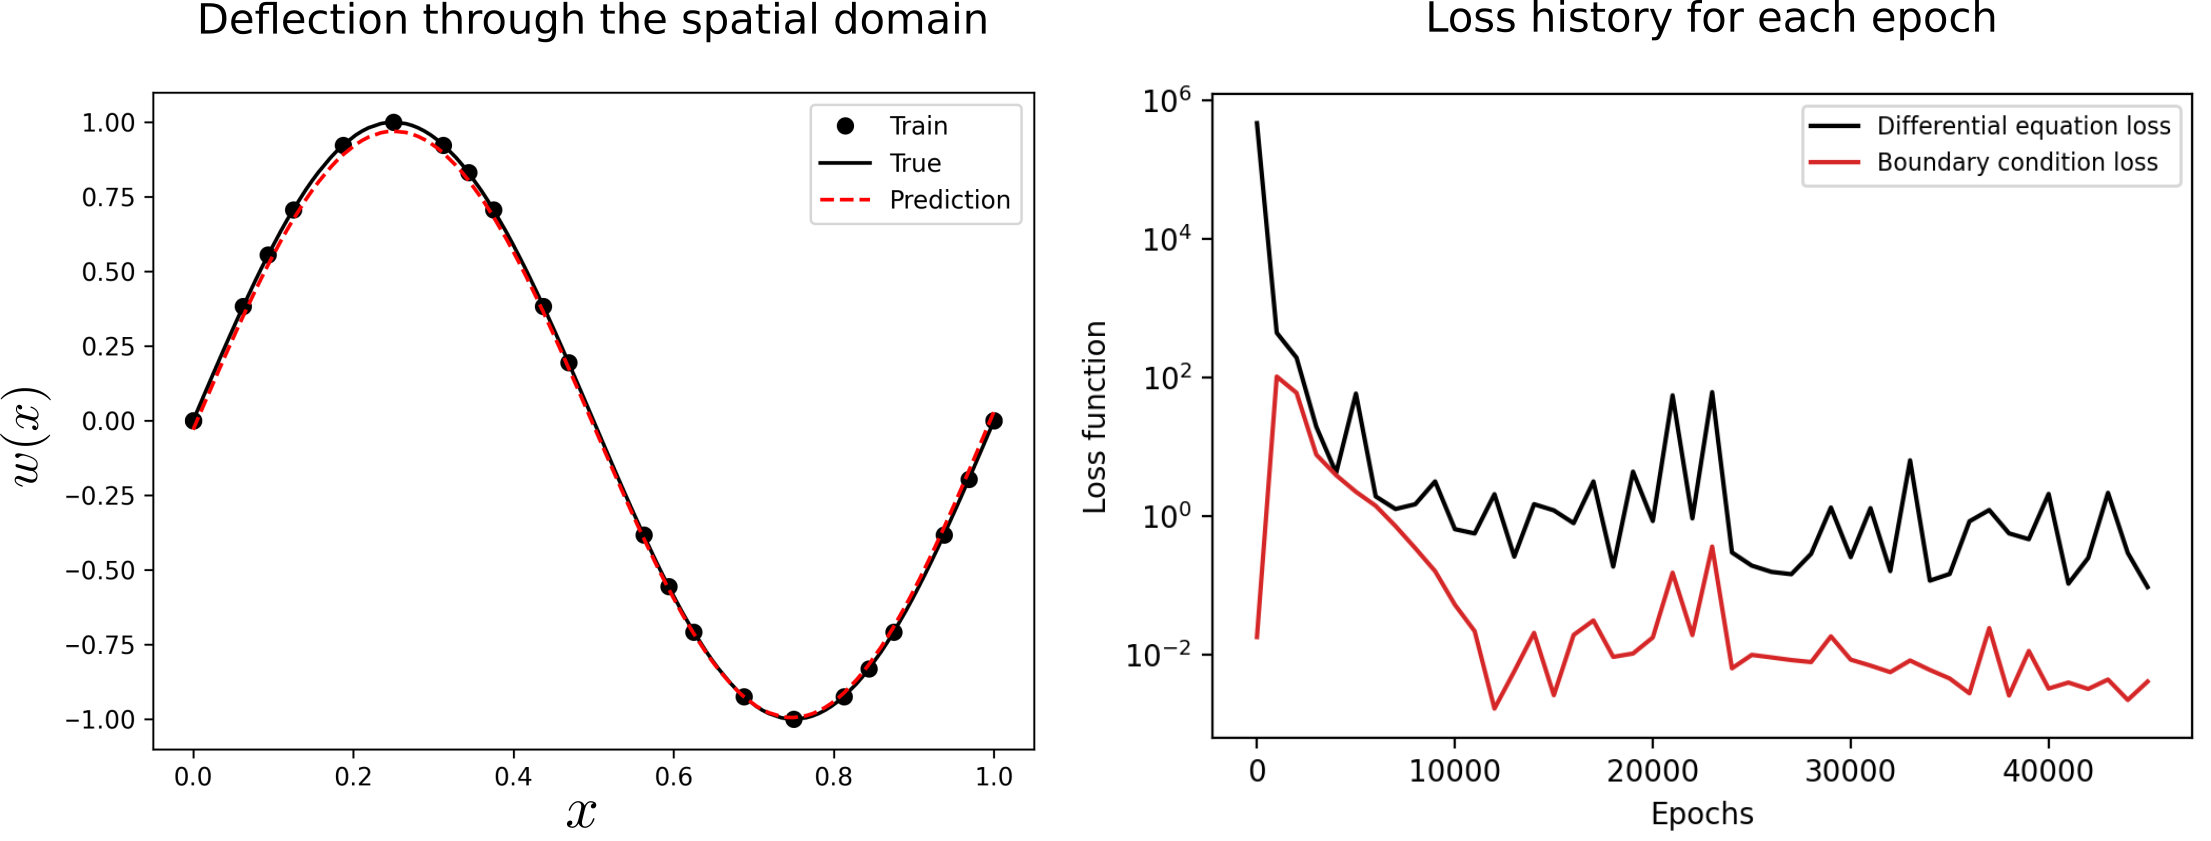
\includegraphics[scale=0.6]{static_res_complex.png}  
    \caption{On the figure left, the predicted and true deflection through the
    spatial domain are represented. On the figure right, the
    loss history containing the differential equation and boundary condition losses
    are given for each epoch.}
    \label{fig:res_complex}
\end{figure}


\section{Continuous-Time Model}

Involving the time term to the Euler beam theory transforms the problem into a vibration problem and 
the behavior of the beam is governed by the Euler-Lagrange equation. The partial differential equation
of the one-dimensional Euler-Lagrange beam including Neumann and Dirichlet boundary conditions 
with initial conditions is formulated as 

\begin{equation}
    \label{eq:dynamic_beam_1}
    \rho A \frac{\partial^{2} w(x,t)}{\partial t^{2}} + \frac{\partial^{2}}{\partial x^{2}}\left(E I \frac{\partial^{2} w(x,t)}{\partial x^{2}}\right) + q(x, t) = 0 \quad \text{ on } \mathcal{T} \otimes  \Omega
\end{equation}

\begin{equation}
    \label{eq:dynamic_beam_2}
    \frac{\partial w(x,t)}{\partial x} = h \quad \text { on } \mathcal{T} \otimes \Gamma_{N},
\end{equation}

\begin{equation}
    \label{eq:dynamic_beam_3}
    w(x,t) = g \quad \text { on } \mathcal{T} \otimes \Gamma_{D},
\end{equation} 

\begin{equation}
    \label{eq:dynamic_beam_4}
    w(x,0) = g_{0} \quad \text{and} \quad w_{t}(x,0) = g_{t,0} \quad \text { on } \Omega.
\end{equation} 

Here, in addition to the spatial domain $\Omega$ in the static models, the temporal domain $\mathcal{T}$ is introduced. 
To give a better understanding, the spatial domain is defined $\Omega = [0,L=1]$, 
with $\Gamma_{D}= \{x | x = 0, x = 1\}$ and $\Gamma_{N}= \{x | x = 0, x = 1\}$ and 
the temporal domain i set to $\mathcal{T}=[0,1]$. Since the beam is particularly considered as a clamped support
Euler-Lagrange beam, the following homogenous boundary conditions are subjected to the problem 

\begin{equation}
    \begin{aligned}
    \label{eq:dynamic_beam_bc}
    w(0,t)=0 & \quad \text{and} & w_{x}(0,t)=0, \\
    w(1,t)=0 & \quad \text{and} & w_{x}(1,t)=0,
    \end{aligned}
\end{equation}

\vspace{5mm}
\noindent with the following non-homogenous initial conditions 

\begin{equation}
    \label{eq:dynamic_beam_ic}
    w(x,0)=\sin(\pi x) \quad \text{and} \quad w_{t}(x,0)=0.
\end{equation}

Similarly, physics-informed neural network approximates the unknown solution $w(x,t)$ using the spatial domain $x$ 
and temporal domain $t$ as inputs as illustrated in Fig. \ref{fig:pinn_dynamic_beam}. Since the predicted solution
has to fulfill the governing equation of Euler-Lagrange problem, residuum $f$ is defined as

\begin{equation}
    \label{eq:f_dynamic}
    f:=\rho A \frac{\partial^{2} w(x,t)}{\partial t^{2}} + \frac{\partial^{2}}{\partial x^{2}}\left(E I \frac{\partial^{2} w(x,t)}{\partial x^{2}}\right) + q(x, t).
\end{equation}

Combining Eqs. \ref{eq:dynamic_beam_bc}, \ref{eq:dynamic_beam_ic}, \ref{eq:f_dynamic} with \ref{eq:total_loss_compact}, 
\ref{eq:total_loss}, \ref{eq:Neumann_pinn}, \ref{eq:Dirichlet_pinn}, \ref{eq:Initial_pinn}, \ref{eq:res_loss}, the loss
function $L$ of a dynamic clamped supported Euler-Lagrange beam is derived as

\begin{equation}
    \label{eq:app_dynamic_overall_loss}
    \begin{aligned} 
        L & = E_{Neumann} + E_{Dirichlet} + E_{0} + E_{f} \\ 
          & = \frac{1}{N_{b}} \sum_{i=1}^{N_{b}}\left[\left(\frac{\partial}{\partial x} w_{P}\left(x_{b}^{i},t_{b}^{i}\right)-h\right)^{2} +
          \left( w_{P}\left(x_{b}^{i},t_{b}^{i}\right)-g\right)^{2} \right] + \\
          & \quad \; \frac{1}{N_{0}} \sum_{i=1}^{N_{0}}\left[\left(\frac{\partial}{\partial t} w_{P}\left(x_{0}^{i},0\right)-g_{t,0}\right)^{2} +
          \left( w_{P}\left(x_{0}^{i},0\right)-g_{0}\right)^{2} \right] + 
          \frac{1}{N_{f}} \sum_{i=1}^{N_{f}}\left(f_{P} (x_{f}^{i},t_{f}^{i})\right)^{2} \\
          & = \frac{1}{N_{b}} \sum_{i=1}^{N_{b}}\left[\underbrace{\left(\frac{\partial}{\partial x} w_{P}\left(x_{b}^{i},t_{b}^{i}\right)\right)^{2}}_{\text{Neumann BC.}} +
          \underbrace{ \vphantom{\left(\frac{\partial}{\partial x}\right)} \left( w_{P}\left(x_{b}^{i},t_{b}^{i}\right)\right)^{2}}_{\text{Dirichlet BC.}} \right] + \\
          & \quad \; \frac{1}{N_{0}} \sum_{i=1}^{N_{0}}\left[\underbrace{ \left(\frac{\partial}{\partial t} w_{P}\left(x_{0}^{i},0\right)-\sin (\pi x)\right)^{2} +
          \left( w_{P}\left(x_{0}^{i},0\right)\right)^{2}}_{\text{Initial C.}} \right] +  
          \frac{1}{N_{f}} \sum_{i=1}^{N_{f}}\left(f_{P} (x_{f}^{i},t_{f}^{i})\right)^{2}
    \end{aligned}
\end{equation}

While the Neumann and Dirichlet loss terms enforces the boundary conditions at $N_{b}$ random points 
$\left\{x_{b}^{i},t_{b}^{i}\right\}_{i=1}^{N_{b}}$ where $x=0$ and $x=1$, the initial loss terms enforce the initial conditions at 
$\left\{x_{0}^{i},0\right\}_{i=1}^{N_{0}}$, since the temporal domain is set to $t_{b}=0$. Finally, the last term assures 
that the predicted displacement fulfills the governing equation of the problem at random $N_{f}$ collocation points
$\left\{x_{f}^{i},t_{f}^{i}\right\}_{i=1}^{N_{f}}$ where the spatial domain $x \in [0,1]$ and the temporal domain $t \in [0,1]$. 


\begin{figure}[!ht]
    \centering
    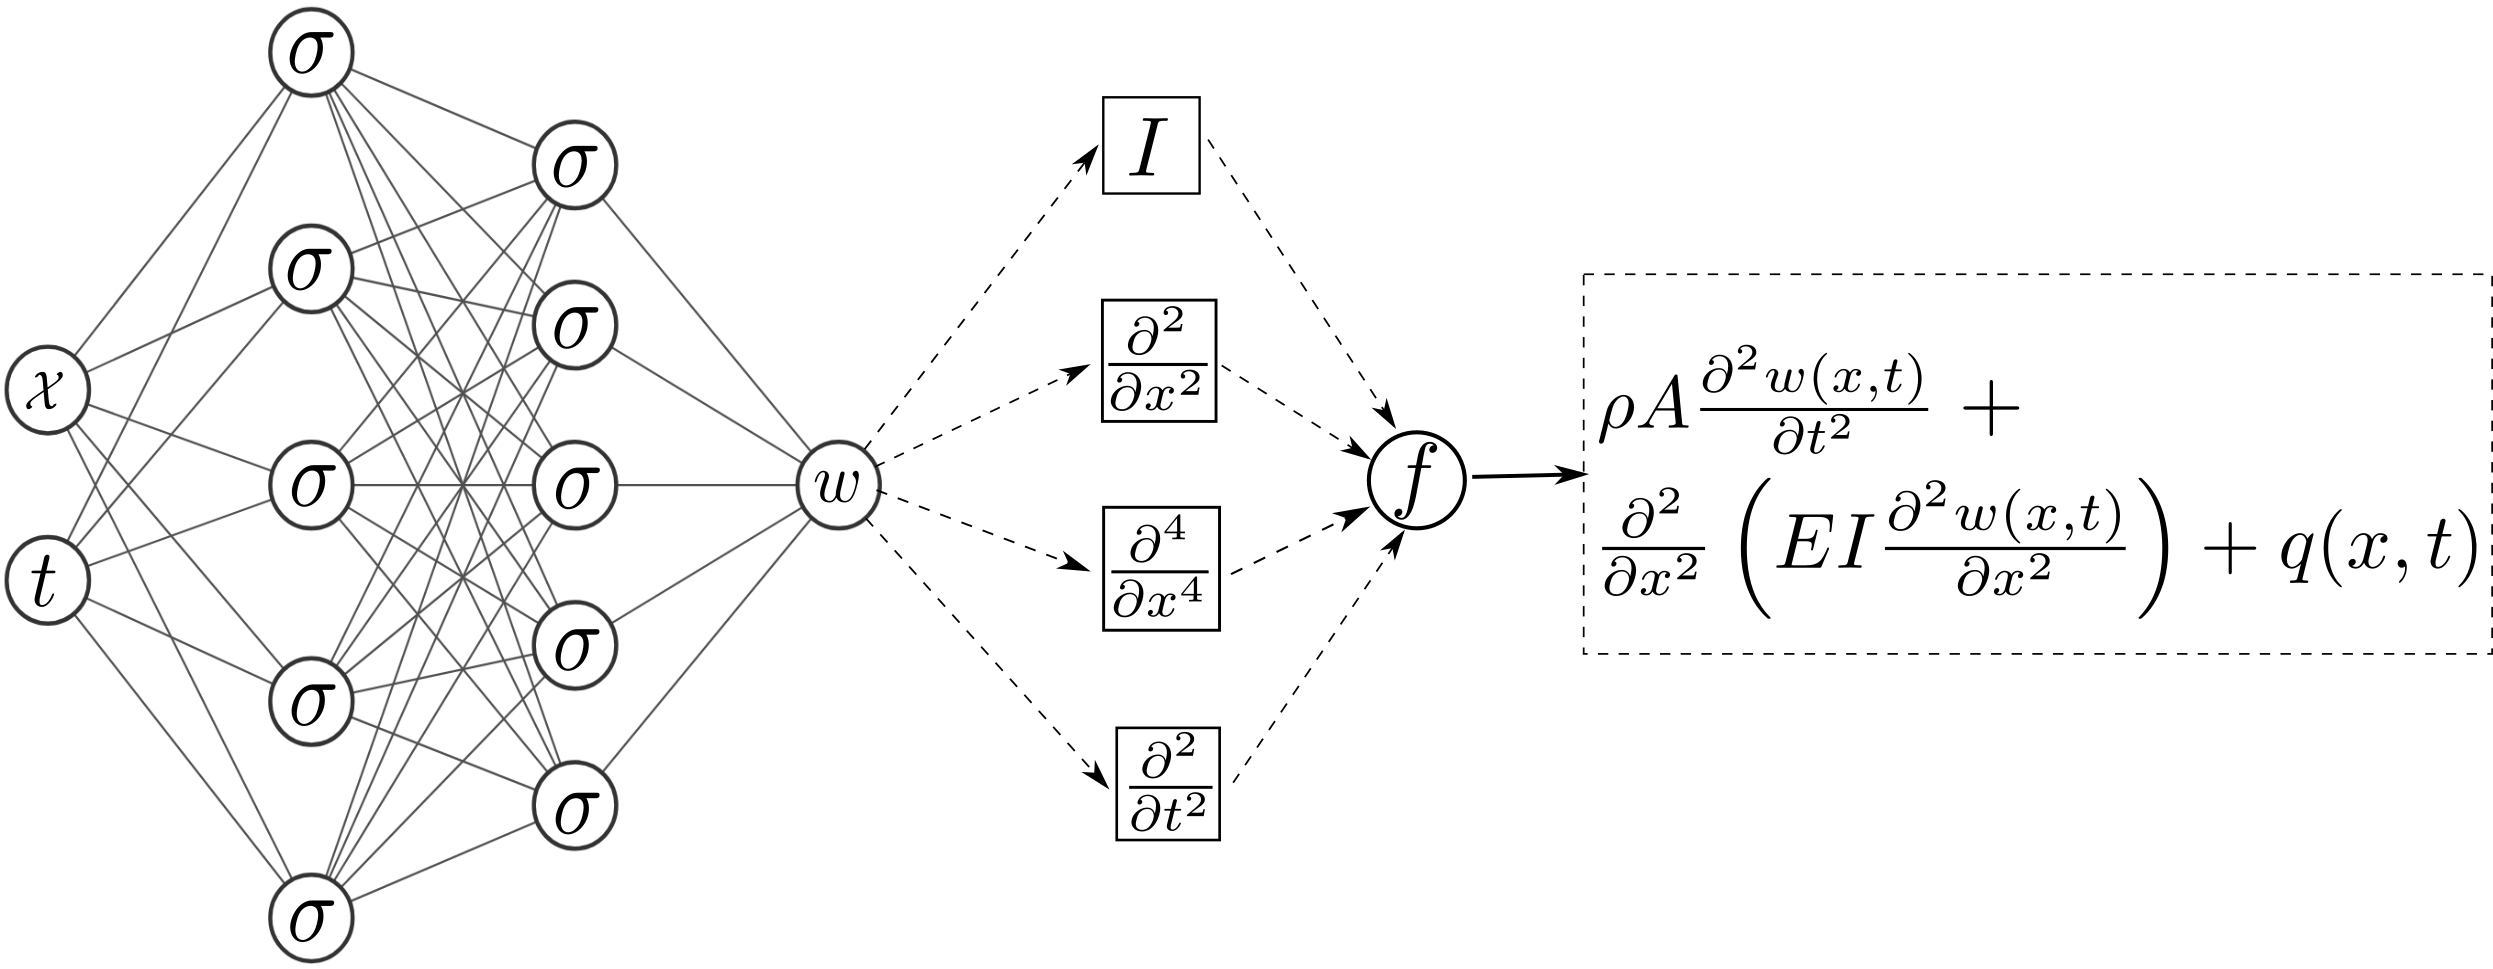
\includegraphics[scale=0.6]{pinn_dynamic_beam.png}  
    \caption{An illustration of physics-informed neural network for the governing
    partial differential equation of the one-dimensional Euler-Lagrange beam.}
    \label{fig:pinn_dynamic_beam}
\end{figure}


The further calculation of the continuous-time model of the Euler-Lagrange beam, Young’s modulus
and the moment of inertia terms are set to $AE = 1$ and additionally the density and the area of the cross-section terms 
are set to $\rho A=1$. Applying the following distributed load

\begin{equation}
    \label{eq:force_time}
    q(x,t) = sin(\pi x) e^{-t} \left( \pi^{4}(t+1)+t-1 \right), 
\end{equation}

\noindent results in the analytical solution of the clamped Euler-Lagrange beam with the given boundary 
and initial conditions (see \ref{eq:dynamic_beam_bc} and \ref{eq:dynamic_beam_ic}) as follows

\begin{equation}
    \label{eq:time_analytical}
    w(x,t) = \sin(\pi x)(t+1) e^{-t}.
\end{equation}


Compared to the PINN architecture of static models, a slightly more advanced model is generated since the input has two dimensions.
The PINN architecture to predict the space-time solution $w(x,t)$ has the following features

\begin{itemize}
    \item Architecture contains 2 input layers, 1 output layer and 3 hidden layers
    containing 100 nodes.
    \item Similarly Hyperbolic tangent activation functions $tanh$ are used with $Glorot Uniform$ initializer.
    \item The $Adam$ optimizer with learning rate $l_{r}=0.0001$ is chosen as the optimization method. 
    The number of $epochs$ is set as 20000. 
    \item The number of collocation points inside domain is set to $N_{f} = 20$, the number of boundary condition points is set
    to $N_{b}=50$ and the number of initial condition point is set to $N_{0}=50$. Additionally, the $Sobol$ sampling
    is performed have a random distribution.
\end{itemize}

The results of the Euler-Lagrange beam is given in Fig. \ref{fig:beam_time_res}. The comparison of the predicted 
and analytical solutions at different space and time intervals shows that the PINN architecture can predict the solution quite well
if the time term is kept constant. On the other hand, the predicted and analytical solutions have a small gap if the space term
is taken as constant. To fill this gap, the model is trained longer or the parameters of the PINN architecture are optimized using
hyper-parameter optimization techniques.


\begin{figure}[ht]
    \centering
    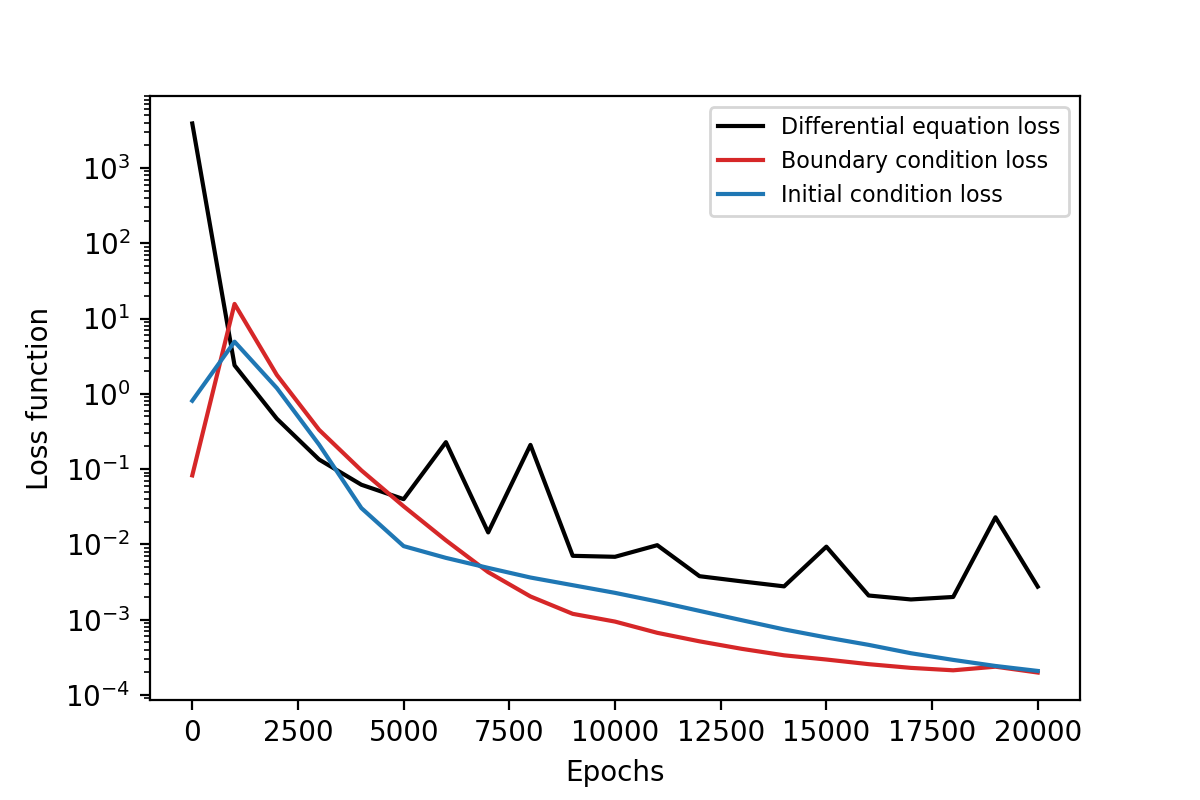
\includegraphics[scale=0.48]{case_2_time.png}  
    \caption{The loss history containing
    the differential equation and boundary condition losses are given for each epoch.}
    \label{fig:beam_time_loss}
\end{figure}

In contrast to the static models, the overall loss contains also the initial condition loss as depicted in Fig. \ref{fig:beam_time_loss}. 
The loss on the known conditions have a smooth decay to the convergence level, while the differential equation loss has local oscillations
due to the difference in magnitudes of order since the small changes in the predicted solution can lead to relatively large
oscillations during the training.  

%\iffalse
%\begin{figure}[!hb]
%    \centering
%    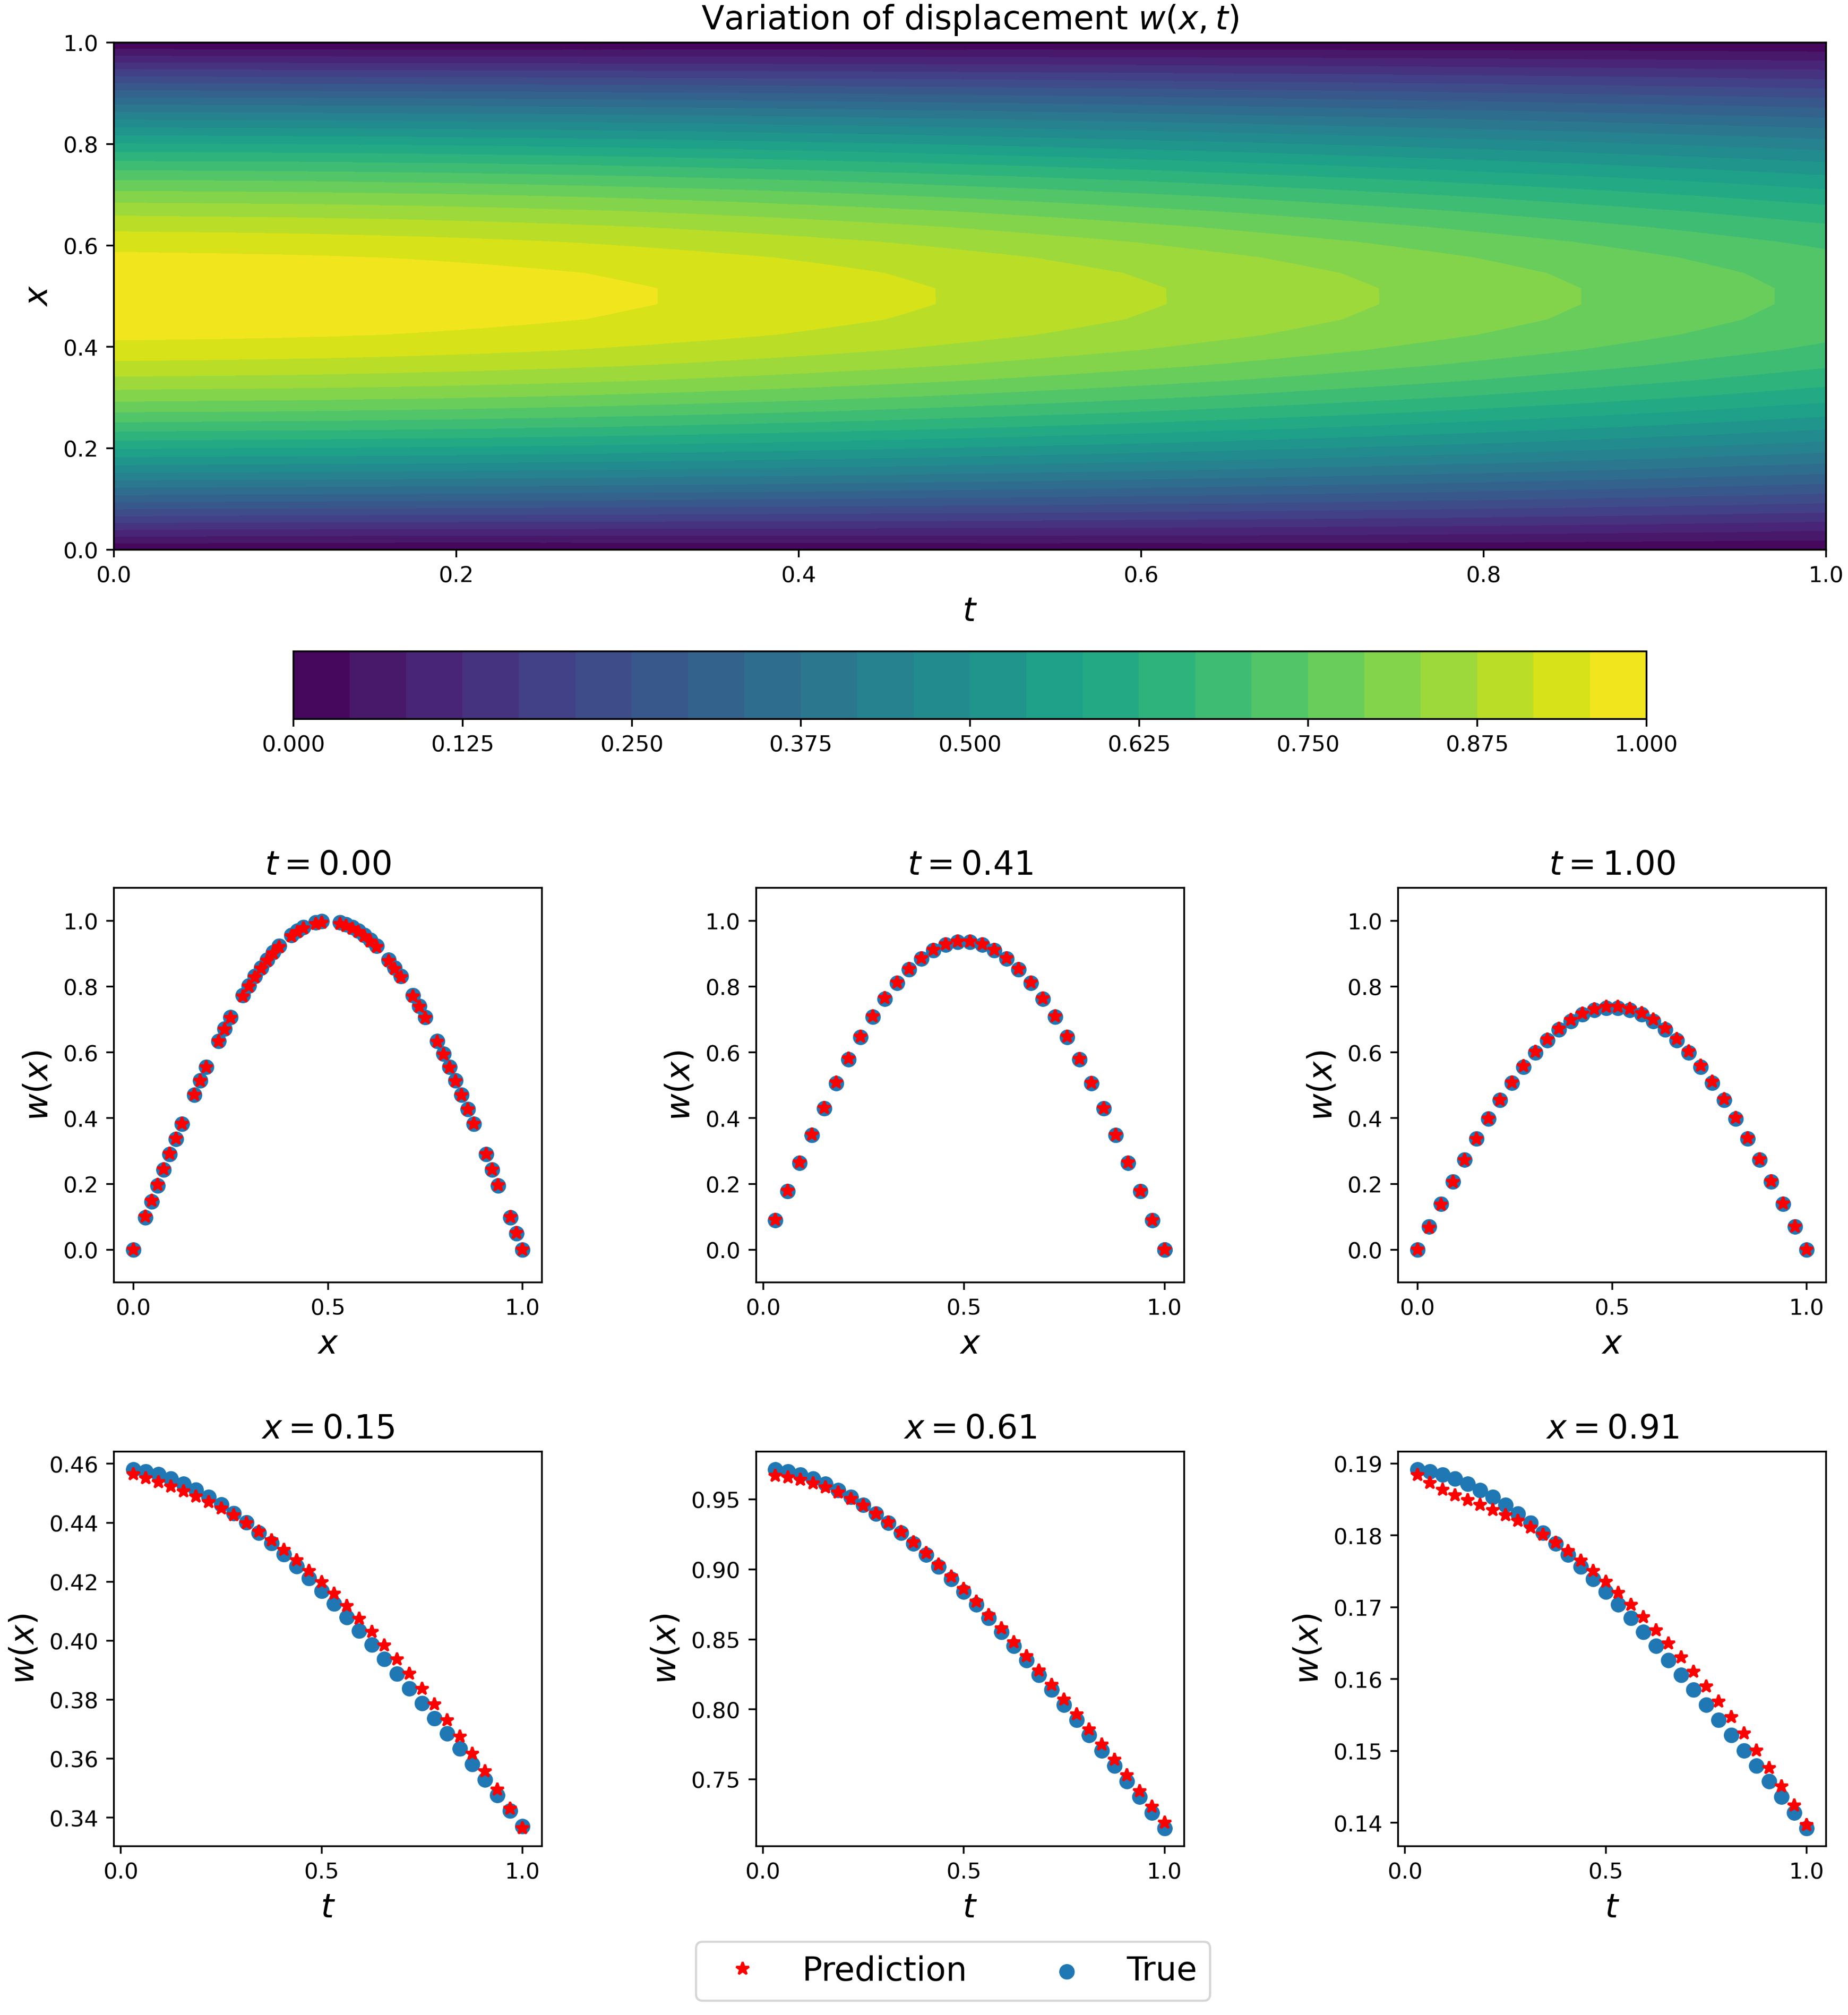
\includegraphics[scale=0.4,trim={1cm 2cm 20cm 5cm},clip]{beam_combined.png}  % 
%    \caption{AAA.}
%    \label{fig:beam_time_res}
%\end{figure}
%\fi
\begin{figure}[b]
    \centering
    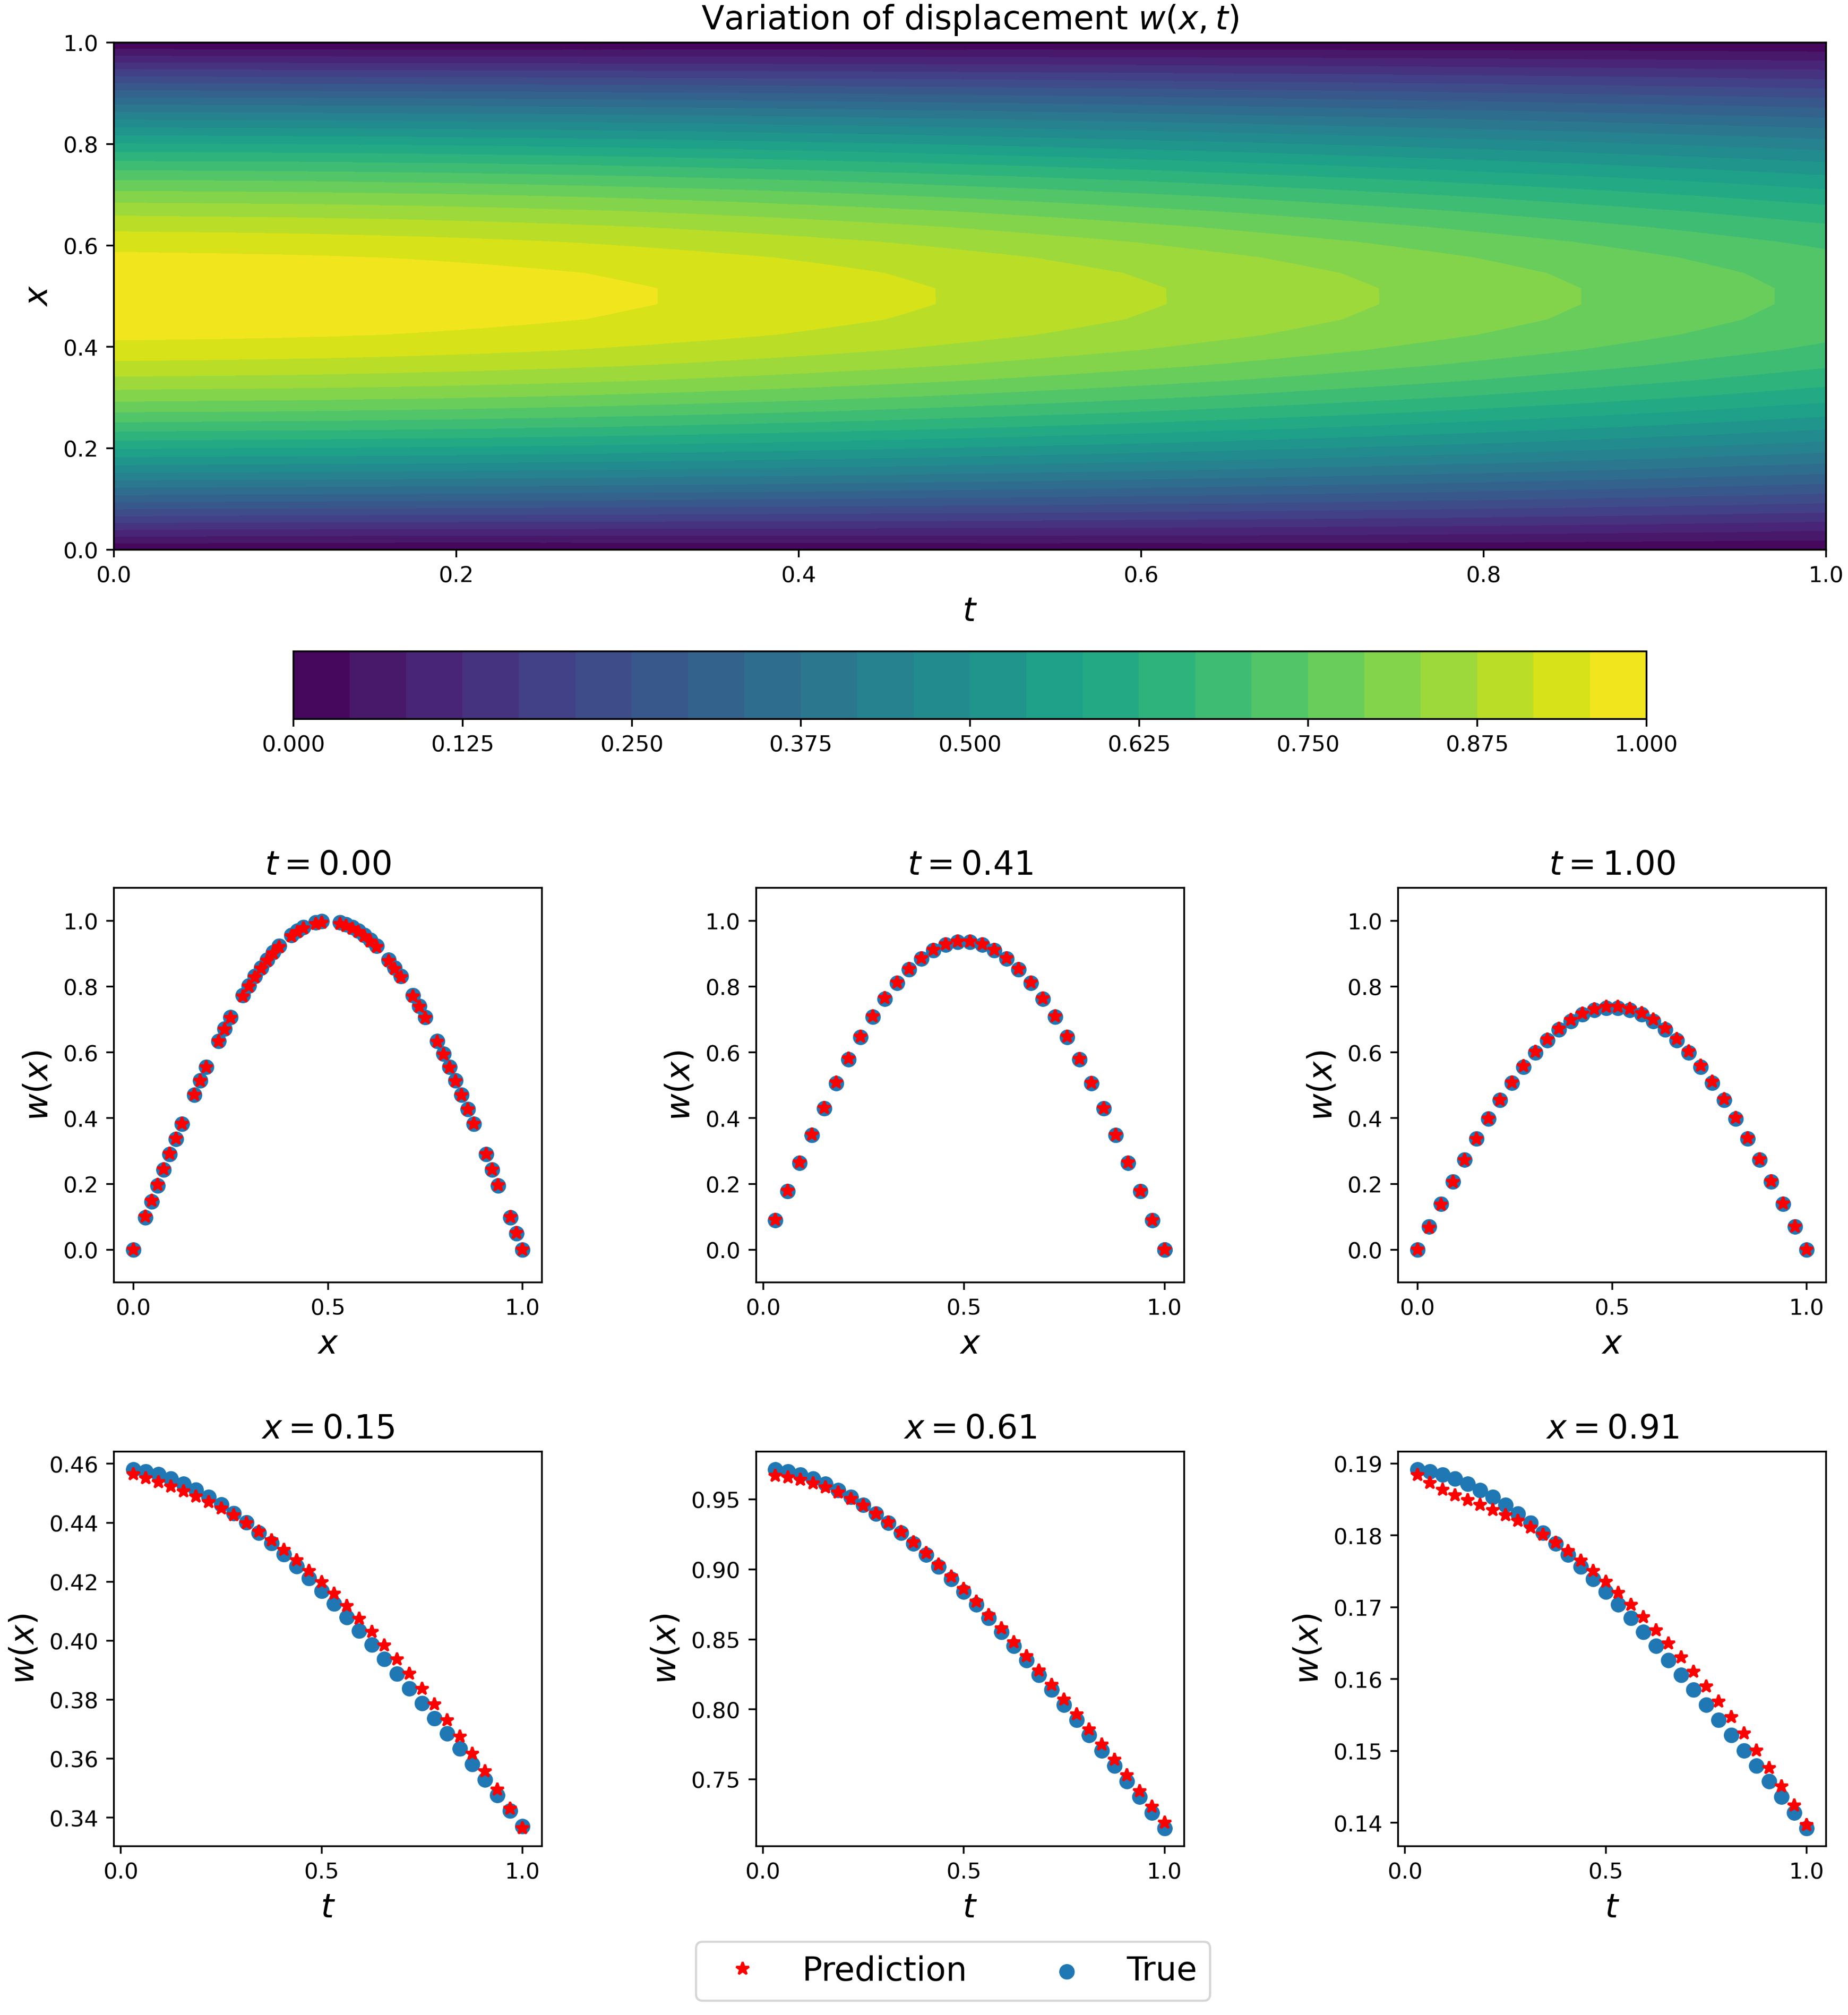
\includegraphics[scale=0.38]{beam_combined.png}
    \caption{The results of the Euler-Lagrange beam. The figure with the colorbar gives the predicted solution through the space-time domain.}
    \label{fig:beam_time_res}
\end{figure}


 % PINNs on beam examples
    %\chapter{Conclusion}
\label{sec:fourth}


 % Conclusion

    %\appendix           % "Chapter" is renamed "Appendix"
    %\appendixpage       % Similar to \part*{Appendices}, but appears in TOC.

    %\chapter{The First Appendix}
\label{sec:first-app}
\kant[20-21] % Dummy text
\section{First Section}
\kant[22]    % Dummy text
\section{Second Section}
\kant[23-24] % Dummy text
    %\chapter{The Second Appendix}
\label{sec:second-app}
\kant[25-29] % Dummy text

    \backmatter         % Folios in Arabic numerals, unnumbered chapters.

    \printbibliography

\end{document}